% Journal of Complex Networks initial-review manuscript.
% Standard article.cls; text block follows the journal's 30 x 46 pica rule.
\documentclass[10pt,a4paper]{article}

\usepackage[T1]{fontenc}
\usepackage{lmodern}
\usepackage[textwidth=126mm,textheight=195mm,centering]{geometry}
\usepackage{graphicx}
\usepackage{amsmath,amssymb,amsfonts,amsthm,bm}
\usepackage{booktabs,tabularx,array}
\usepackage{xcolor}
\usepackage{url}
\usepackage{microtype}
\usepackage[numbers,sort&compress]{natbib}
\usepackage[toc]{appendix}
\usepackage[section]{placeins}
\usepackage{hyperref}

\hypersetup{
  pdftitle={Testing Algorithmically Mediated Social Hysteresis: Closed-Loop Causal Tests and Reversal Control},
  pdfauthor={Simone D'Agnano},
  pdfsubject={Computational social science; adaptive networks; recommender systems; reversal controllability},
  pdfkeywords={social hysteresis, algorithmic mediation, adaptive networks, recommender systems, causal identification, reversal controllability},
  colorlinks=true,
  linkcolor=blue,
  citecolor=blue,
  urlcolor=blue
}

\raggedbottom
\setlength{\emergencystretch}{3em}
\newcommand{\alphamax}{\alpha_{\max}}
\newcommand{\Gup}{G_{\uparrow}}
\newcommand{\Gdown}{G_{\downarrow}}
\newcommand{\dd}{\mathrm{d}}
\newcommand{\E}{\mathbb{E}}
\newcommand{\R}{\mathbb{R}}
\newcommand{\inlinehead}[1]{\par\smallskip\noindent\textbf{#1}\ }
\newcolumntype{Y}{>{\raggedright\arraybackslash}X}
\newcommand{\alttext}[1]{\par\smallskip\noindent\textit{Alt text:} #1}

\newtheorem{proposition}{Proposition}
\newtheorem{lemma}{Lemma}
\newtheorem{definition}{Definition}
\newtheorem{remark}{Remark}
\renewcommand{\arraystretch}{1.18}
\setlength{\arrayrulewidth}{0.45pt}

\title{Testing Algorithmically Mediated Social Hysteresis:\\
Closed-Loop Causal Tests and Reversal Control}
\author{Simone D'Agnano\\
\small Dipartimento di Scienze e Innovazione Tecnologica (DISIT),\\
\small Universit\`a del Piemonte Orientale, Viale Teresa Michel 11,\\
\small 15121 Alessandria, Italy\\
\small \href{mailto:s.dagnano.research@gmail.com}{s.dagnano.research@gmail.com}\\
\small \href{https://orcid.org/0009-0003-6394-9408}{ORCID 0009-0003-6394-9408}}
\date{}

\begin{document}
\maketitle
\begin{abstract}
Withdrawal asymmetry, social hysteresis, and recommender feedback are prior ideas, not novelty claims of this paper. The unresolved problem is how to identify a history effect at matched current algorithmic mediation, distinguish it from finite-rate relaxation, and determine which admissible interventions reverse the resulting state. We index potential outcomes by complete randomized policy histories and separate finite-rate path dependence, rate-robust path dependence, rejection of a declared relaxation class, model-dependent quasistatic persistence, and quasistatic hysteresis as a system property. A constructive impossibility baseline proves that any finite collection of graded histories and marginal observations is compatible with both a globally monostable latent system and a multistable discrete-time Markov system when latent dimension and relaxation are unrestricted. For a prespecified class of Markov kernels with unique invariant laws and uniform Wasserstein contraction, we derive mean branch-gap bounds for step-and-dwell and continuous ramps, together with a prospective vacuity gate. We separate total-system, candidate-standardized, reset-sensitive, and channel-attributable estimands. Reversal deficit compares path closure and endpoint restoration with a contemporaneous low-mediation reference; vector-valued costs define a Pareto-minimal policy set. Exact equilibrium reduction, tangential-root safeguards, full-Jacobian stability analysis, grid refinement, and independent adaptive integration audit the normal form. A second model uses bidirectional degree-preserving rewiring across 32 initializations; a finite-horizon Poisson bound links bridge repair to reverse-mixing capacity. A gatekept cluster-randomized program executes the proposed reassignment statistic inside every power replicate and separates platform-state restoration from human recovery. Together, these results turn algorithmically mediated social hysteresis from a qualitative possibility into a falsifiable causal program that separates randomized history effects, relaxation-class rejection, and reversal control. The framework tests these claims without presuming that any real platform exhibits quasistatic hysteresis.
\end{abstract}

\noindent\textbf{Keywords:} social hysteresis, algorithmic mediation, adaptive networks, recommender systems, causal identification, reversal controllability

\section{Introduction}

Bak-Coleman et al. already identify hysteresis as a reason why short withdrawal need not invert prior social-media exposure, and show why feedback, evolving network structure, scale, and interference complicate conventional randomized-trial interpretations \cite{bakcoleman2025actionable,bakcoleman2025rct}. We therefore treat treatment--state non-equivalence as a premise rather than a novelty claim:
\begin{equation}
\boxed{\text{restoring the treatment is not equivalent to restoring the state}.}
\label{eq:principle}
\end{equation}
Equality of current treatment is a design condition. Restoration of the social, network, and algorithmic state is an estimand.

One experimentally tractable diagnostic object is not a single contrast between ``algorithmic'' and ``chronological'' feeds, but a closed control path,
\begin{equation}
0\longrightarrow\alphamax\longrightarrow0,
\end{equation}
and the question whether
\begin{equation}
\Gup(\alpha)\neq\Gdown(\alpha)
\end{equation}
at matched current policy. In the locked synthetic protocols below, policy equality is implemented by the same numerical value of a platform-defined mediation control $\alpha$; in an experiment it additionally requires the same versioned ranking, interface, moderation, and exposure mapping.

Prior work establishes social and recommender hysteresis; our contribution is therefore methodological rather than phenomenological. Hysteresis in social systems and adaptive networks is established \cite{sznajdweron2024toward,oestereich2020hysteresis,nowak2020threshold,macy2021polarization,su2017contagion,chen2019vaccine,graham2020sociology,maia2021adaptive,asikainen2020cumulative}. Zeng et al. already demonstrated an explicit hysteresis effect in a coevolving user--item/recommender system \cite{zeng2015mutual}; Chan proposed multilevel platform hysteresis and recommender resets \cite{chan2026brake}; recommender--opinion feedback and control-theoretic recommender design are also prior work \cite{davidson2026closedloop,depasquale2026control,mariano2026optimal,mariano2026pathological}; and classical identification already uses rate variation, minor loops, return-point memory, and inverse control. This paper does not claim to introduce algorithmic hysteresis, withdrawal asymmetry, closed-loop recommender control, those diagnostics, or minimum-cost control.

This paper addresses the remaining methodological problem: identification, falsification, and reversal under graded algorithmic mediation. For a completely specified graded path, we define current-treatment-matched causal branch contrasts indexed by full randomized policy histories; test branch distributions against a prespecified stochastic relaxation class; and use randomized time-indexed interventions to estimate reversal deficits and cost-constrained recovery policies. The control $\alpha$ is physical and preregistered---for example, the fraction of eligible impressions selected by a locked learned ranker---not an ontological measure of ``AI intensity.''

A 2026 field experiment on X provides a direct empirical motivation. Switching from a chronological to an algorithmic feed changed engagement and several political attitudes, whereas the reverse switch produced no comparable change; follows induced by algorithmic exposure also persisted in the chronological condition \cite{gauthier2026x}. That asymmetry is consistent with the state-restoration problem in Eq.~\eqref{eq:principle}, but it does not identify a loop because the two directions involved different initially selected populations and a binary feed contrast. Conversely, large Meta experiments changed exposure and engagement but found limited or null short-term changes in several political outcomes \cite{guess2023feeds,nyhan2023likeminded,gonzalez2023segregation,guess2023reshares}. A removal experiment can estimate withdrawal from an already altered state while missing the historical effect of constructing that state.

This paper makes five contributions. First, it turns the prior withdrawal-asymmetry concern into complete-history, matched-current-treatment estimands. Second, Lemma~\ref{lem:finite-record-equivalence} supplies a finite-record impossibility baseline, while Proposition~\ref{prop:stochastic-rate-separation} bounds both step-and-dwell and continuous branch distributions for a declared Wasserstein-contracting null. Third, it distinguishes total-system, candidate-standardized, reset-sensitive, and channel-attributable effects. Fourth, reversal deficit and reversal control ask which platform-state restoration policy closes the path and contemporaneous reference-state deficit, at what multidimensional cost. Fifth, two synthetic stress-test families and a staged cluster-randomized design show what would falsify, rather than merely instantiate, the proposed framework. We turn algorithmically mediated social hysteresis from a qualitative possibility into a falsifiable causal program by separating three questions that on/off designs conflate: whether randomized history matters at matched current policy, whether a declared finite-rate relaxation class can explain the branch gap, and which admissible interventions restore the resulting state. None of these finite-rate objects is relabeled as identified quasistatic hysteresis.

\section{Claim boundary and literature map}

\subsection{Social hysteresis, tipping, and irreversibility}

Hysteresis is stronger than persistence. Persistence means that an outcome changes slowly. Hysteresis means that the input-output relation is history-dependent, typically with coexistence of responses over an interval of the control parameter. In social systems, the concept has been formalized using threshold, Ising-like, kinetic-opinion, and agent-based models \cite{sznajdweron2024toward,nowak2020threshold,oestereich2020hysteresis,macy2021polarization}. Network contagion can generate discontinuous adoption and hysteresis loops \cite{su2017contagion}; controlled experiments have also demonstrated tipping of established social conventions after a committed minority crosses a critical mass \cite{centola2018tipping}. The broader tipping literature emphasizes that abrupt transitions, critical slowing, and hysteresis are related but not interchangeable diagnostics \cite{scheffer2009warning,wiedermann2020threshold}.

Two recent precedents are particularly close. The expressed-private-opinion model of Kami\'nska and Sznajd-Weron ties collective hysteresis to dissonance reduction \cite{kaminska2025cognitive}. Cruz-Castillo and Cozzo obtain saddle-node structure and hysteresis in public expression on clustered homophilic networks \cite{cruzcastillo2026spiral}. Neither makes the mediation intensity of a learned recommender the cycled control or decomposes platform, topological, and human memory under matched algorithmic exposure. This paper addresses that missing inferential step.

\subsection{Adaptive networks already store social history}

Adaptive networks couple dynamics \emph{on} a graph with dynamics \emph{of} the graph \cite{gross2008adaptive}. The literature includes coevolving voter models, bounded-confidence systems, rewiring under homophily, and fragmentation transitions \cite{holme2006nonequilibrium,kozma2008consensus,gil2006coevolution,vazquez2008adaptive,kan2023adaptive,li2025adaptive}. Asikainen et al. show that triadic closure combined with homophily can store the memory of earlier homophilic constraints, explicitly interpreting it as hysteresis \cite{asikainen2020cumulative}; this is the closest topological-memory predecessor to Model II. Foundational opinion models show how assimilation, bounded confidence, and biased processing generate consensus, fragmentation, or polarization \cite{deffuant2000mixing,castellano2009statistical,dandekar2013assimilation}. Empirical and mechanistic work connects unfollowing, homophily, socio-cognitive bias, and community structure to echo chambers \cite{sasahara2021unfollowing,wang2020public,cinelli2021echo}. Models with nonlinear interaction or multidimensional topics further show that more interaction need not monotonically reduce disagreement \cite{baumann2020echo,baumann2021topics,thurner2025interactions}.

Accordingly, the novelty is not that adaptive networks can store history, but how such history can be causally identified and reversed under algorithmic mediation. A changed follow graph is already a valid memory substrate. Algorithmic mediation becomes scientifically distinctive when one identifies how ranking, profile learning, and algorithmically induced topology alter a closed-path response beyond a human-only or static-network baseline.

\subsection{Relation to classical hysteresis identification and control}

Classical hysteresis identification supplies several diagnostics used here but not invented here. Preisach and Prandtl--Ishlinskii operators represent rate-independent input--output memory through elementary switching or play operators; Bouc--Wen and Duhem families provide differential descriptions with rate-dependent and rate-independent limits \cite{preisach1935magnetic,macki1993mathematical,hassani2014survey,oh2005duhem}. Minor loops probe nested state dependence, while return-point memory is a stronger, model-contingent property rather than a generic consequence of hysteresis \cite{sethna1993hierarchies,mungan2019returnpoint}. Identification and inverse-control methods estimate or compensate these operators under controlled inputs \cite{krejci2001inverse,ikhouane2007systems}.

The social-platform setting adds causal assignment, evolving topology, interference, learned profiles, creator response, and ethically non-resettable human states. We therefore import rate variation, minor loops, and reversal tests as diagnostics, while locating the residual contribution in their randomized causal implementation. Rejecting a declared relaxation class is not equivalent to identifying a Preisach, Bouc--Wen, or any other specific hysteresis operator.

\subsection{Algorithmic opinion dynamics and recommender feedback}

Models of algorithmic filtering show that personalization can change opinion distributions and that its effects depend on network correlations, friendship rewiring, posting, limited attention, and content-selection rules \cite{perra2019personalisation,sirbu2019bias,arruda2022algorithms,peralta2020asymmetry,valensise2023drivers,donkers2024desounding}. Rossi, Polderman, and Frasca explicitly formulated a closed loop between opinion formation and personalized recommendation \cite{rossi2018closedloop}; Davidson and Ye model the reciprocal recommender--opinion loop directly \cite{davidson2026closedloop}. More recent work studies optimal control of ranking in heterogeneous modular systems and the mechanistic coupling among limited memory, reposting, rewiring, recommendation, and polarization \cite{gezha2026control,oliveira2026interplay}. Recommender systems have also been formalized as control systems, including long-horizon fairness interventions and state-feedback control over networked opinions \cite{depasquale2026control,mariano2026optimal,mariano2026pathological}. People recommenders can also change network exposure and polarization, so ``feed ranking'' is only one mediation surface \cite{cinus2022people}.

A parallel recommender-systems literature studies data--algorithm feedback. Repeated recommendations can confound inferred preferences, homogenize behavior, amplify popularity or preference, and alter network structure \cite{chaney2018confounding,mansoury2020feedback,kalimeris2021amplification,zhao2013longterm,su2016network}. Induced-preference and algorithmic-drift work explicitly models longitudinal preference change under recommendation, and network-aware feedback optimization already connects recommender control to evolving opinions \cite{coppolillo2025drift,chandrasekaran2026networkaware}. Natural experiments and comparative evaluations show that recommender effects depend on objective, topology, and user response rather than following a universal direction \cite{moller2018diversity,fabbri2022minorities,frey2010connections}. Proposed remedies include exploration, causal adjustment, and deconvolution \cite{jadidinejad2020exploration,krauth2025causal,sinha2016deconvolving}. Long-run evaluation remains underdeveloped because short-horizon accuracy can miss collective effects \cite{jannach2020mcnamara,ge2020ecommerce,zoralioglu2026dynamic}.

Bak-Coleman et al. are the closest conceptual-causal predecessor: they explicitly connect withdrawal asymmetry to hysteresis, network persistence, feedback, and SUTVA violations \cite{bakcoleman2025actionable}. Zeng et al. are the closest direct dynamical predecessor \cite{zeng2015mutual}: their coevolving bipartite network exhibits direction-dependent stationary item-popularity inequality when recommendation bias is swept. Chan's Research Note is the closest multilevel platform conjecture \cite{chan2026brake}. The remaining gap is not the intuition but the combination of a graded randomized path, full-history estimand, stochastic rate-null rejection, and time-indexed restoration policy. Table~\ref{tab:closest} makes this boundary explicit.

\begin{table}[!htbp]
\centering
\caption{Closest predecessors and the remaining inferential gap.}
\label{tab:closest}
\footnotesize
\setlength{\tabcolsep}{3pt}
\renewcommand{\arraystretch}{0.94}
\begin{tabularx}{\textwidth}{|p{2.6cm}|Y|Y|Y|}
\hline
\textbf{Study} & \textbf{Control and state} & \textbf{Established contribution} & \textbf{Remaining gap addressed here}\\
\hline
Bak-Coleman et al. (2025; v3 2026) & Withdrawal and feature changes in a coupled social-media system & Withdrawal asymmetry, hysteresis, network persistence, and SUTVA critique & No graded randomized loop, matched-branch full-history estimand, rate-null rejection, or timed restoration\\
\hline
Zeng et al. (2015) & Bias sweep in a coevolving user--item network; popularity Gini & Recommender-system hysteresis and incomplete reversal of popularity concentration & No randomized matched-history social-state estimand, rate separation, reset localization, or reversal criterion\\
\hline
Asikainen et al. (2020) & Triadic closure and homophily in an adaptive network & Topological memory of prior homophilic constraints, linked to hysteresis & No mediation coordinate, complete-history experiment, or reversal policy\\
\hline
Davidson--Ye; De Pasquale et al.; Mariano--Frasca (2026) & Recommender--opinion dynamics and feedback control & Closed-loop dynamics and optimal-control formulations & No randomized matched-branch identification or path/state reversal deficit\\
\hline
Chan (2026) & Feedback at user, platform, and market levels & Multilevel hysteresis conjecture; breaks and resets proposed as tests & No quantitative closed path, network simulation, causal identification, or intervention frontier\\
\hline
Gauthier et al. (2026) & Binary algorithmic/chronological feed switches on X & Asymmetric causal effects and persistent algorithm-induced follows & Different initial populations; no graded loop or randomized restoration\\
\hline
This study & Graded histories with randomized path, rate, and restoration & Total-system/controlled estimands, relaxation bound, reversal deficit, and staged inference & Prospective implementation required; numerical and power results are synthetic\\
\hline
\end{tabularx}
\end{table}

\subsection{Empirical evidence is mixed for principled reasons}

Audits and experiments establish that algorithms can change exposure. Twitter's ranking amplified political content in a large randomized system comparison \cite{huszar2022amplification}; observational studies document ideological exposure patterns on Facebook and across online news pathways \cite{bakshy2015exposure,flaxman2016bubbles}; audits find ranking differences on Twitter and partisan exposure skews on TikTok \cite{bandy2021twitter,ibrahim2026tiktok}. Counterfactual-bot work on YouTube demonstrates that recommendation effects can be estimated against controlled viewing paths and need not always point toward extremity \cite{hosseinmardi2024youtube}.

Effects on attitudes are more contingent. Search-ranking experiments, collaborative-filtering environments, and exposure to opposing partisans can move outcomes, sometimes in counterintuitive directions \cite{cho2020search,neumann2023curation,bail2018opposing}. A browser-based reranking intervention changed affective polarization, and a custom-feed experiment changed perceived partisan norms \cite{piccardi2025reranking,brady2026norms}. At the same time, high-powered field experiments report precisely estimated nulls for several outcomes \cite{guess2023feeds,nyhan2023likeminded,guess2023reshares}. Social influence itself is well established in large online experiments \cite{muchnik2013influence,bond2012mobilization}, but deactivation studies show that platform-level welfare and political consequences vary by endpoint and period \cite{allcott2024deactivation}.

Reviews therefore caution against a monocausal ``algorithm causes polarization'' narrative \cite{kubin2021review,vanbavel2021shapes,hartmann2025review,mahmoudi2024review}. The correct hypothesis is conditional: particular objectives, interfaces, populations, network structures, and histories can generate path dependence. Causal-recommender and platform-economics reviews similarly emphasize feedback, confounding, incentives, and long-run outcomes \cite{gao2024causal,ge2024trustworthy,aridor2024economics}. Opinion-dynamics surveys provide model families, not a substitute for identification \cite{noorazar2020survey}.

\section{Definitions and falsifiable estimands}

Let the cluster-level policy at time $t$ be
\begin{equation}
p_{ct}=\{\alpha_{ct},\mathcal Q_{ct},\mathcal R_{ct},R_{ct}\},
\end{equation}
where $\alpha$ is a platform-specific mediation control, $\mathcal Q$ is the candidate-generation rule, $\mathcal R$ is the ranking rule, and $R$ is a restoration or recovery intervention. An interpretable $\alpha$ is the fraction of eligible impressions selected by a locked learned ranker rather than a specified baseline. It is a physical control coordinate, not a universal measure of ``algorithmic intensity.''

The primitive potential outcome is indexed by the complete vector of assigned policy histories,
\begin{equation}
Y_{ict}\!\left(\bm{\bar p}_{0:t}\right).
\label{eq:full-history-po}
\end{equation}
This notation includes run-in, dwell times, previous maxima, cycle count, minor loops, candidate and ranking versions, restoration timing, and the histories of other clusters. Under a correct exposure mapping,
\begin{equation}
Y_{ict}\!\left(\bm{\bar p}_{0:t}\right)
=Y_{ict}\!\left(\bar p_{c,0:t},\bar e_{ic,0:t}\right),
\qquad
\bar e_{ic,0:t}=\phi_{ic,t}\!\left(\bm{\bar p}_{-c,0:t},W\right),
\label{eq:exposure-map}
\end{equation}
where $W$ contains baseline variables only. Branch, rate, and current mediation do not by themselves define a treatment. Only after every path feature is fixed by protocol do we use $G_{\uparrow}^{(v)}(\alpha)$ and $G_{\downarrow}^{(v)}(\alpha)$ as shorthand for expectations of Eq.~\eqref{eq:full-history-po}. Because treatment can itself alter the interference network, observed post-treatment cross-cluster exposure is treated as a diagnostic or outcome of assigned policy unless a sequential causal model explicitly justifies conditioning on it; it is not silently inserted into the baseline exposure map.

Let $G$ be a preregistered bounded scalar outcome or one component of a vector outcome. The signed branch gap and two area summaries are
\begin{align}
\Delta_G^{(v)}(\alpha)
  &=G_{\downarrow}^{(v)}(\alpha)-G_{\uparrow}^{(v)}(\alpha),\\
\mathcal H_G^{\mathrm{signed}}(v)
  &=\int_{0}^{\alphamax}\Delta_G^{(v)}(\alpha)\,\dd\alpha,\\
\mathcal H_G^{\mathrm{abs}}(v)
  &=\int_{0}^{\alphamax}|\Delta_G^{(v)}(\alpha)|\,\dd\alpha.
\end{align}
Area is defined relative to the preregistered physical coordinate $\alpha$ and is not invariant to a monotone reparameterization. It is therefore not intrinsically comparable across platforms. Every analysis also reports the branch function, maximum absolute gap, and endpoint deficit.

\inlinehead{Finite-rate path dependence.} $\Delta_G^{(v)}(\alpha)\neq0$ somewhere at an observed rate. This is the minimal design-based empirical claim.

\inlinehead{Rate-robust path dependence.} A branch discrepancy persists across a preregistered finite range of rates. This remains compatible with an arbitrarily slow monostable process outside that range.

\inlinehead{Relaxation-class rejection.} The observed branch discrepancy is incompatible with a prespecified relaxation class $\mathfrak L$ under a valid class-rejection test. This result rejects that explanation; it does not by itself identify bistability or quasistatic hysteresis.

\inlinehead{Quasistatic hysteresis.} Distinct ascending and descending branch limits persist as $v\rightarrow0$ under explicit existence and interchange-of-limit assumptions. No finite experiment nonparametrically proves this limit.

\inlinehead{Algorithmically induced history effect.} A randomized complete algorithmic policy history changes $G$ at matched current policy. This total-system effect may operate through realized candidate supply, ranking, profiles, topology, creator response, or human state.

\inlinehead{Reset-sensitive history effect.} A randomized restoration policy changes the history contrast. Channel attribution additionally requires a surgical, reference-emulating intervention, exclusion of direct reset effects, support, and control of regeneration. Without those assumptions the identified object is a policy interaction, not a mediated effect.

Minor loops and return-point tests are classical diagnostics rather than novelty claims. Reversing $\alpha$ before $\alphamax$ and reversing again probes previous-maximum dependence; nested closure or systematic failure of return-point memory constrains mechanism geometry.

\begin{figure}[!htbp]
\centering
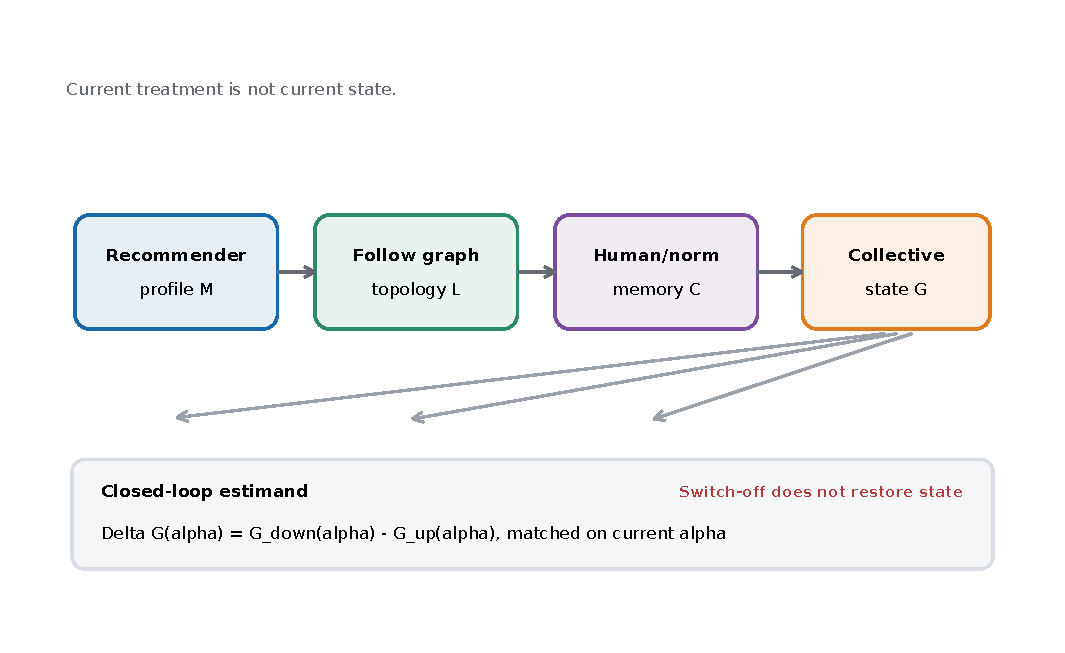
\includegraphics[width=\textwidth]{Fig1.pdf}
\caption{The current mediation setting is not a sufficient state variable. Algorithmic exposure can leave information in recommender profiles, the follow graph, and human or normative states. The branch contrast matches the contemporaneous value of $\alpha$ while varying its history.}
\label{fig:ledger}
\alttext{Four linked state boxes represent recommender profile, follow-graph topology, human or normative memory, and collective state. Arrows show that the same current mediation can be reached with different retained states.}
\end{figure}

\section{Identification and reversal controllability}

\subsection{Why regularity restrictions are necessary}

Randomization can identify the causal response to each assigned finite history without identifying the latent dynamical class that generated those responses. The following lemma strengthens the familiar two-endpoint observation.

\begin{lemma}[Impossibility baseline: finite-record observational equivalence]
Let
\begin{equation}
\mathcal O=\{(a_{i,0:n_i-1},n_i,\nu_i):i=1,\ldots,N\}
\end{equation}
be any finite collection of treatment sequences $a_{i,n}\in[0,1]$ observed at finite discrete update indices $n_i$, together with target marginal outcome laws on a Polish outcome space. Equivalently, the sequences may encode piecewise-constant graded paths sampled at their update boundaries. Assume only finite-record consistency: identical treatment prefixes at an identical observation index have the same target law. Without restrictions on latent dimension, relaxation rate, or the observation kernel, there exist both (i) a controlled Markov system with one globally exponentially attracting invariant state at every fixed treatment and (ii) a controlled system with a nonempty bistable control interval and distinct stable equilibrium branches that starts from a common initial state and reproduces every marginal law in $\mathcal O$ exactly.
\label{lem:finite-record-equivalence}
\end{lemma}

The construction is given in Appendix~A. It covers any finite set of graded histories, rates, discrete observation indices, and minor-loop observations, not only two endpoints. Its scope is equally important: it matches finite marginal laws, not an unrestricted full longitudinal joint law. This is an impossibility baseline, not the positive identification result: a finite record cannot reject the union of all monostable models when arbitrarily slow mixing and unrestricted observation sensitivity are allowed. A useful test therefore requires scientifically defensible regularity restrictions fixed independently of the branch outcomes.

\subsection{A stochastic relaxation null for step-and-dwell and continuous ramps}

Let $(\mathsf X,d_{\mathsf X})$ and $(\mathsf Z,d_{\mathsf Z})$ be Polish metric spaces and $\mathcal P_1$ the laws with finite first moment. For each current mediation $a$, let $P_a$ be a Markov kernel on latent state and $H_a$ a possibly stochastic observation kernel. The latent state must be dynamically sufficient: conditional on $X_n$ and current $a$, transition law $P_a$ has no additional branch, calendar, or earlier-history dependence. Time-varying environments must be randomized-matched or included in $X_n$.

Define the null class $\mathfrak L(q,L_\pi,L_H)$ by four requirements: (S1) $P_a$ has invariant law $\pi_a$; (S2) uniformly in $a$,
\begin{equation}
W_{\mathsf X}(\mu P_a,\mu'P_a)\leq qW_{\mathsf X}(\mu,\mu'),\qquad 0\leq q<1;
\label{eq:wasserstein-contraction}
\end{equation}
(S3) $W_{\mathsf X}(\pi_a,\pi_{a'})\leq L_\pi|a-a'|$; and (S4) the observation kernel is $L_H$-Lipschitz from state to outcome in $W_1$. Uniform contraction implies uniqueness of $\pi_a$. A primitive kernel-continuity bound $\sup_xW_{\mathsf X}\{P_a(x,\cdot),P_{a'}(x,\cdot)\}\leq L_P|a-a'|$ permits the conservative choice $L_\pi=L_P/(1-q)$.

\begin{proposition}[Stochastic branch-distribution bound]
\label{prop:stochastic-rate-separation}
Assume (S1)--(S4). For a step-and-dwell branch $b$, let level $a_{b,k}$ be followed by $m_{b,k}$ transitions under $P_{a_{b,k}}$, so $\mu_{b,k}=\mu_{b,k-1}P_{a_{b,k}}^{m_{b,k}}$. After a fixed-control run-in of $m_0$ transitions with initial distance at most $\rho_b$, define
\begin{align}
R_{b,0}&=q^{m_0}\rho_b,\\
R_{b,k}&=q^{m_{b,k}}\{R_{b,k-1}+L_\pi|a_{b,k}-a_{b,k-1}|\}.
\label{eq:step-recursion}
\end{align}
Then $W_{\mathsf X}(\mu_{b,k},\pi_{a_{b,k}})\leq R_{b,k}$. At matched levels $a_{\uparrow,k}=a_{\downarrow,\ell}=a$, the observed laws $\nu_{b,k}=\mu_{b,k}H_a$ satisfy
\begin{equation}
W_{\mathsf Z}(\nu_{\downarrow,\ell},\nu_{\uparrow,k})
\leq L_H(R_{\downarrow,\ell}+R_{\uparrow,k}).
\label{eq:step-branch-bound}
\end{equation}
If $\rho_b\leq\rho$, every dwell has at least $m$ transitions, and each increment is at most $\delta$, then uniformly
\begin{equation}
B_{\mathrm{step}}=2L_H\!\left\{q^{m_0}\rho+
\frac{q^mL_\pi\delta}{1-q^m}\right\}.
\label{eq:step-uniform-bound}
\end{equation}
For a continuous semigroup satisfying $W(\mu P_a^t,\mu'P_a^t)\leq e^{-\kappa t}W(\mu,\mu')$, assume additionally that along every absolutely continuous path $a_b(t)$ the nonautonomous evolution $U_{s,t}^{a_b}$ exists as the $W_{\mathsf X}$ limit, uniformly on compact time intervals, of the time-ordered piecewise-constant propagators $\prod_jP_{a_b(t_{j-1})}^{t_j-t_{j-1}}$ as the partition mesh tends to zero. Then
\begin{equation}
R_b(t)=\rho_b e^{-\kappa(T_0+t)}+L_\pi\int_0^t e^{-\kappa(t-s)}|\dot a_b(s)|\,\dd s.
\end{equation}
The matched branch-law distance is at most $L_H\{R_\downarrow+R_\uparrow\}$; if $|\dot a_b|\leq v$,
\begin{equation}
B_{\mathrm{cont}}(v,T_0)=2L_H\!\left\{\rho e^{-\kappa T_0}+\frac{L_\pi v}{\kappa}\right\}.
\label{eq:continuous-bound}
\end{equation}
For scalar outcomes with absolute-distance metric, the same bounds apply to differences in means.
\end{proposition}

The proof in Appendix~A uses contraction, invariance, the triangle inequality through the common invariant law, and Kantorovich duality. If one Markov transition lasts $\Delta t$ and each level contains $m$ transitions, the dwell duration is $\Delta T=m\Delta t$. The correct discrete--continuous scaling is
\begin{equation}
q^m=e^{-\kappa\Delta T},\qquad \delta=v\Delta T,
\qquad
\frac{q^mL_\pi\delta}{1-q^m}\longrightarrow\frac{L_\pi v}{\kappa}
\quad(\Delta T\downarrow0).
\end{equation}
Thus the synthetic step-and-dwell protocols can be diagnosed against Eq.~\eqref{eq:step-recursion}; they are no longer compared informally with a theorem for a different control path.

If constants are calibrated rather than fixed as the null definition, let $\mathcal C_{1-\eta}$ be a prespecified joint confidence set for $\vartheta=(q,L_\pi,L_H,\rho)$ or $(\kappa,L_\pi,L_H,\rho)$ and set
\begin{equation}
\overline B_j=\sup_{\vartheta\in\mathcal C_{1-\eta}}B_j(\vartheta).
\label{eq:lag-envelope}
\end{equation}
For the primary scalar outcome, let $\underline D_j$ be simultaneous lower limits for $|\E Z_{\downarrow,j}-\E Z_{\uparrow,j}|$. Reject the class only if $\max_j(\underline D_j-\overline B_j)>0$; the false class-rejection probability is at most $\eta+\gamma$. This mean-based test follows directly from Kantorovich--Rubinstein duality and avoids claiming that a high-dimensional empirical $W_1$ distance has been estimated precisely. A direct branch-law $W_1$ test on a prespecified low-dimensional outcome remains an optional stronger analysis. Calibration arms or sample splitting prevent branch outcomes from tightening their own null.

Operationally, $j$ indexes every preregistered combination of matched policy level and rate. If $c_\gamma$ is the randomization-based simultaneous critical value and $\widehat\Delta_j\pm c_\gamma\widehat{\mathrm{SE}}_j$ are simultaneous two-sided intervals, then
\begin{equation}
\underline D_j=\max\{0,|\widehat\Delta_j|-c_\gamma\widehat{\mathrm{SE}}_j\},
\qquad
\text{reject }\mathfrak L\text{ if }\max_j(\underline D_j-\overline B_j)>0.
\label{eq:simultaneous-lower-bound}
\end{equation}
The construction controls selection over all locked level--rate cells rather than only the visually largest gap.

\inlinehead{Prospective vacuity gate.} If the outcome-space diameter is $D_Z$, the test is vacuous whenever $\overline B\geq D_Z$. For $Z\in[0,1]$, $L_H=\rho=1$, $L_\pi=0.5$, $\kappa_L=0.20$, $T_0=20$, and $v=0.005$, Eq.~\eqref{eq:continuous-bound} gives $\overline B\simeq0.062$. Holding the other values fixed but allowing $\kappa_L=0.02$ gives $\overline B\simeq1.59$, which is untestable on $[0,1]$. The class-rejection arm does not estimate an unrestricted physical mixing rate: it tests a substantive null class defined by external lower bounds on relaxation and upper bounds on input and observation sensitivity. Those bounds must come from prior experiments, engineering constraints, stationary calibration arms, or a blinded pilot whose outcomes cannot tighten the tested envelope. If no nonvacuous, externally defensible joint set can be fixed---including when it admits $q=1$ or $\kappa=0$---Stage~2 is not run and no relaxation-class rejection claim is made. Network summaries may also induce a prohibitively large $L_H$.

Exceeding the envelope rejects only the prespecified class of systems with a unique invariant law, uniform Wasserstein contraction, and the declared input and observation regularity. Alternatives include polynomial mixing, near-critical slowing, metastability, omitted state, calendar nonstationarity, misspecified interference, or genuine multistability. It does not by itself establish bistability or a nonzero quasistatic limit.

The claim ladder is therefore fixed throughout the paper:
\begin{equation}
\begin{aligned}
&\text{randomized history effect}
  \Rightarrow \text{finite-rate path dependence},\\
&\text{persistence over tested rates}
  \Rightarrow \text{rate-robust path dependence},\\
&\text{rejection of prespecified }\mathfrak L
  \not\Rightarrow \text{quasistatic hysteresis},\\
&\text{model-dependent persistence as }v\to0
  \Rightarrow \text{quasistatic hysteresis},\\
&\hspace{8em}\text{under the declared model assumptions}.
\end{aligned}
\label{eq:claim-ladder}
\end{equation}
The arrows are evidential escalation, not logical equivalences. In particular, relaxation-class rejection is named as such and is never used as a synonym for hysteresis identification.

\begin{table}[!htbp]
\centering
\caption{Identification supplied by each experimental component.}
\label{tab:identification}
\small
\begin{tabularx}{\textwidth}{|p{3.2cm}|Y|Y|}
\hline
\textbf{Design component} & \textbf{Identified object} & \textbf{What remains unresolved}\\
\hline
Randomized complete histories at matched current policy & Total-system history contrast at the tested schedule & Dynamical class and mediation mechanism\\
\hline
Closed path plus stationary controls & Loop geometry; diagnosis and adjustment of common calendar drift & Arbitrarily slow relaxation without a mixing restriction\\
\hline
Multiple randomized rates & Empirical rate law and rejection of a declared stochastic envelope & Quasistatic limit and alternatives outside the class\\
\hline
Verified randomized restoration $R$ & Reset-sensitive history interaction and deficit change & Channel attribution without surgical exclusion and reference emulation\\
\hline
Replicated cycles and minor loops & Repeatability, accommodation, and return-point diagnostics & A unique microscopic memory mechanism\\
\hline
\end{tabularx}
\end{table}

\subsection{Reversal deficit and cost-constrained reversal policies}

Closing a signed loop is not equivalent to restoring a state: positive and negative branch gaps can cancel, and both branches can converge to the same altered endpoint. Let $\bm Z$ contain the primary outcome and the algorithmic, network, or human states whose restoration matters. For an admissible reversal bundle $R$, define
\begin{align}
D_{\mathrm{path}}(R;v)
&=\int_0^{\alphamax}w(\alpha)
d\!\left\{\mathcal L(\bm Z_{\downarrow}^{(v)}(\alpha\mid R)),
\mathcal L(\bm Z_{\uparrow}^{(v)}(\alpha))\right\}\,\dd\alpha,
\label{eq:path-deficit}\\
D_{\mathrm{state}}(R;v,T)
&=d\!\left\{\mathcal L(\bm Z_{\mathrm{end}}^{\mathrm{cycle},R}(T)),
\mathcal L(\bm Z_{\mathrm{ref}}^{\alpha=0}(T))\right\},
\label{eq:state-deficit}
\end{align}
where the reference is a contemporaneous randomized stationary low-mediation arm and $d$ is a preregistered distance. It is not a historically never-treated state: participants may have years of prior platform exposure. The pair $\bm D_R=(D_{\mathrm{path}},D_{\mathrm{state}})$ is the \emph{reversal deficit}. It distinguishes an open return path from \emph{false closure}, in which the branches agree but the endpoint remains far from the experimental low-mediation counterfactual.

\begin{definition}[Reversal controllability]
Let $\mathcal A_R$ be the ethically and technically admissible reversal policies. Each policy has a disclosed cost vector
\begin{equation}
\bm c(R)=(c_{\mathrm{technical}},c_{\mathrm{privacy}},c_{\mathrm{burden}},
c_{\mathrm{welfare}},c_{\mathrm{network}})
\end{equation}
and componentwise budgets $\bm B$. Let $(\epsilon_{\mathrm p},\epsilon_{\mathrm s})$ be prespecified tolerances and define the feasible set
\begin{equation}
\begin{aligned}
\mathcal F_\epsilon(v,T)=\{R\in\mathcal A_R:\;&
\bm c(R)\preceq\bm B,\quad D_{\mathrm{path}}(R;v)\leq\epsilon_{\mathrm p},\\
&D_{\mathrm{state}}(R;v,T)\leq\epsilon_{\mathrm s}\}.
\end{aligned}
\end{equation}
A system is reversal-controllable at $(v,T)$ if $\mathcal F_\epsilon(v,T)\neq\varnothing$. When Pareto-minimal elements exist---in particular, for the finite admissible policy lattice used in the primary design, or under compactness of $\mathcal A_R$, closedness of $\mathcal F_\epsilon$, and lower semicontinuity of every cost coordinate---the primary solution is the Pareto-minimal set
\begin{equation}
\mathfrak R^{\mathrm{Pareto}}_\epsilon(v,T)=
\left\{R\in\mathcal F_\epsilon:\nexists R'\in\mathcal F_\epsilon
\text{ with }\bm c(R')\preceq\bm c(R),\ \bm c(R')\neq\bm c(R)\right\}.
\label{eq:minimum-reversal-bundle}
\end{equation}
Each component lies in $\mathbb R_+$ and must be expressed in a preregistered unit or normalized to a disclosed common scale before scalarization. Only if $\bm\omega\in\mathbb R_+^5$, $\bm\omega\neq\bm0$, is preregistered---with $\sum_k\omega_k=1$ after unit-free normalization---do we define
\begin{equation}
c_{\bm\omega}(R)=\bm\omega^\top\bm c(R),\qquad
\mathfrak R^\star_{\epsilon,\bm\omega}(v,T)=
\arg\min_{R\in\mathcal F_\epsilon(v,T)}c_{\bm\omega}(R).
\end{equation}
\end{definition}

The optimization form is standard target control; the contribution claimed here is the social-history target and the paired path/state deficit, not Pareto optimization. The feasible or Pareto set may be empty or non-unique. Scalar minimum cost is distinct from inclusion minimality and depends transparently on $\bm\omega$. If exact reversal is infeasible, the estimand is the Pareto frontier in $(\bm c,D_{\mathrm{path}},D_{\mathrm{state}})$. Deficit need not be monotone in bundle inclusion: a policy can induce reactance, change candidate supply, accelerate relearning, or remove stabilizing ties.

Profile and topology policies $(M,L)$ are \emph{platform-state restoration}. Deliberation, norm correction, washout support, or counter-attitudinal exposure aimed at $C$ are \emph{human recovery facilitation}: new experiences, not erasure of a person. Primary reversal controllability is defined on technically controllable platform states. Human recovery is reported separately under welfare constraints and cannot be placed on the same semantic intervention lattice without explicit justification.

\subsection{Causal estimands, candidate evolution, and reset separation}

The time-unrolled structural model separates candidate generation from ranking:
\begin{align}
\mathcal K_{ict}&=f_t^K(S_{ct},\alpha_{ct},\mathcal Q_{ct},E_{ict},W,U^K_{ict}),
\label{eq:scm-candidates}\\
\mathcal D_{ict}&=f_t^D(\mathcal K_{ict},M_{it},\alpha_{ct},\mathcal R_{ct},W,U^D_{ict}),\\
S_{c,t+1}&=f_t^S(S_{ct},\mathcal D_{ct},E_{ct},W,U^S_{c,t+1}),\\
Y_{ict}&=f_t^Y(S_{ct},\mathcal D_{ict},E_{ict},W,U^Y_{ict}).
\label{eq:scm}
\end{align}
Here $W$ is measured before history assignment; realized candidates, creator response, follow topology, and learned profiles are post-treatment states. Holding candidate-generation \emph{rules} fixed does not hold realized sets fixed:
\begin{equation}
\mathcal Q_t^\uparrow=\mathcal Q_t^\downarrow
\quad\not\Rightarrow\quad
\mathcal K_{ict}^\uparrow=\mathcal K_{ict}^\downarrow.
\end{equation}

The primary total-system history effect at a matched protocol point is
\begin{equation}
\tau_j^{\mathrm{sys}}(e)=
\E\{Y_{t_j}(h_j^\downarrow,e)-Y_{t_j}(h_j^\uparrow,e)\},
\label{eq:total-system-effect}
\end{equation}
with candidates, slates, profile, topology, creator supply, and human state allowed to evolve. A second intervention may draw candidates from a preregistered history-blind law $\Lambda$, defining the candidate-standardized effect $\tau_j^{K\text{-}\mathrm{ctrl}}(e;\Lambda)$. Its positivity condition is substantive: every item or item stratum assigned positive mass by $\Lambda(\cdot\mid W)$ must be eligible, observable, and safely deliverable under every compared history at that protocol point. The preferred implementation freezes an ex-ante audit reservoir before history assignment and restricts $\Lambda$ to its common-support subset. If only the intersection of history-specific supports is available, $\Lambda$ must be restricted to that intersection and the resulting narrower estimand reported. Assigning mass outside common support is extrapolation, not candidate-standardized causal identification. Candidate replay is not a balance check; it changes the estimand. The difference $\tau^{\mathrm{sys}}-\tau^{K\text{-}\mathrm{ctrl}}$ is a diagnostic policy contrast, not a natural mediated effect without sequential mediation assumptions.

For restoration bundle $J$ randomized at $t_r$, write $\mu_j(h,e,r_J)=\E\{Y_{t_j}(h,e,r_J)\}$. The residual history effect and reset attenuation are
\begin{align}
\tau_j^{H\mid R_J}(e)&=\mu_j(h^\downarrow,e,r_J)-\mu_j(h^\uparrow,e,r_J),\\
A_{J,j}(e)&=\tau_j^H(e)-\tau_j^{H\mid R_J}(e).
\label{eq:reset-attenuation}
\end{align}
$A_{J,j}$ is identified as a history-by-restoration interaction when both assignments are randomized. Calling it channel-attributable further requires reference emulation, exclusion of direct restoration effects, state support, and no history-dependent bypass or regeneration.

\begin{table}[!htbp]
\centering
\caption{Causal estimands and the claims they support.}
\label{tab:estimands}
\small
\begin{tabularx}{\textwidth}{|p{2.5cm}|Y|Y|Y|}
\hline
\textbf{Estimand} & \textbf{Intervention} & \textbf{Allowed to evolve} & \textbf{Interpretation}\\
\hline
Total-system history & Randomized complete paths, matched current policy & Candidates, slates, profile, topology, creators, and human state & Intention-to-treat effect of policy history on the evolving system\\
\hline
Candidate-standardized history & Common history-blind candidate law $\Lambda$ & Profile, human state, and non-candidate pathways & History effect under a standardized information surface\\
\hline
Reset-sensitive history & Randomized $R_J$ within randomized histories & Every unreset state and allowed regeneration & History-by-restoration policy interaction; no mediation claim required\\
\hline
Channel-attributable intervention & Surgical replacement $S^J(t_r)\sim\nu_J^{h'}$ & Prespecified non-$J$ states & Attribution only with exclusion, reference emulation, support, and correct timing\\
\hline
\end{tabularx}
\end{table}

\begin{figure}[!htbp]
\centering
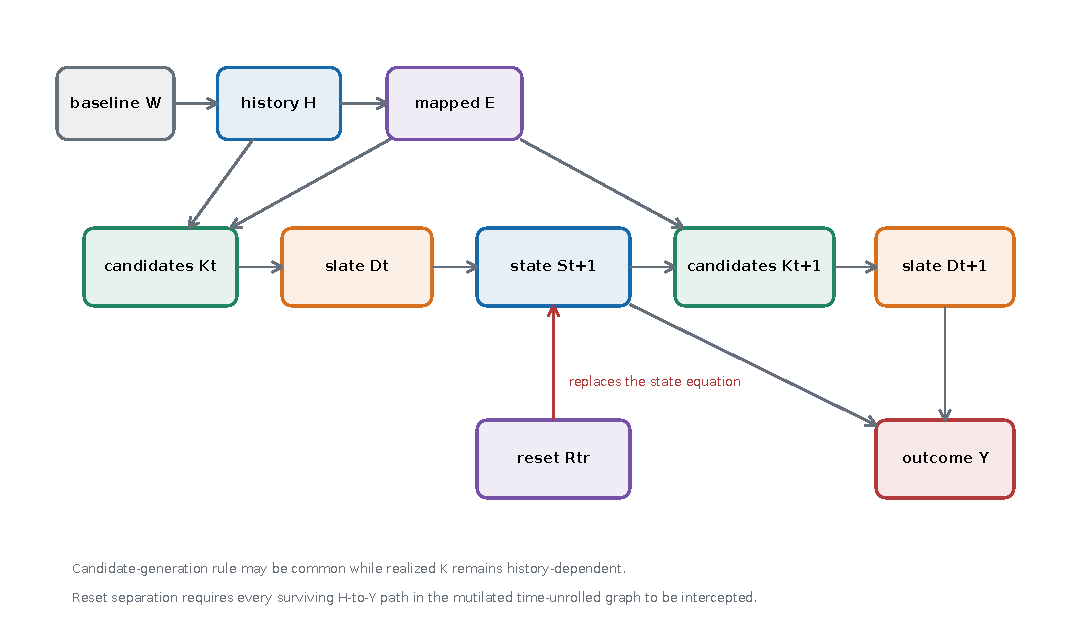
\includegraphics[width=\textwidth]{Fig2.pdf}
\caption{Time-unrolled causal structure. Baseline $W$ precedes randomized history $H$; mapped cross-cluster exposure $E$, realized candidates $\mathcal K$, ranked slates $\mathcal D$, and social/platform state $S$ evolve over time. A reset replaces a time-indexed state equation; it does not erase information already transmitted downstream.}
\label{fig:causal-dag}
\alttext{A time-unrolled directed acyclic graph links baseline variables and randomized history to exposure, candidate sets, ranked slates, evolving state, and outcome. A reset node replaces one state equation, while other history-to-outcome paths remain visible.}
\end{figure}

The graphical implication below is a standard d-separation consequence once a valid intervention cuts every surviving directed path. Its role here is diagnostic: it states exactly when a platform ``reset'' can be interpreted as history separation and prevents a reset interaction from being relabeled as mediator identification by default.

\begin{proposition}[Reset-separation criterion under mapped interference]
\label{prop:reset-separation}
Consider the SCM in Eqs.~\eqref{eq:scm-candidates}--\eqref{eq:scm}. Assume: (i) $W$ precedes assignment and contains no descendant of $\bm H$; (ii) complete-history and restoration assignments are randomized conditional on $W$; (iii) consistency and positivity hold for complete histories, exposure strata, and restoration versions; (iv) interference is restricted by the preregistered mapping $E_i=\phi_i(\bm{\bar p}_{-c},W)$ of the complete policy histories of other clusters; (v) compared histories share post-restoration input, interface, moderation, candidate-generation rule, and ranking rule; (vi) restoration replaces the structural equation for each intervened $S^J(t_r)$ by a history-independent kernel $\nu_J^0(\cdot\mid W)$; and (vii) in the resulting time-unrolled SWIG, after fixing $E_i=e$ and the common post-restoration input, every directed path from pre-restoration history $H_c$ to $Y_i(t)$ is intercepted by a restored node whose incoming arrows have been removed. Then for every supported $h,h',e,w$,
\begin{equation}
\mathcal L\{Y_i(t;h,e,r_J)\mid W=w\}
=\mathcal L\{Y_i(t;h',e,r_J)\mid W=w\}.
\label{eq:reset-separation}
\end{equation}
\end{proposition}

Positivity requires $\Pr(H_c=h,E_i=e,R_J=r\mid W=w)>0$ for every analyzed cell. If history and exposure are deterministically coupled, only an allocation-policy average is identified. A channel label is not automatically a hitting set: resetting $L(t_r)$ does not block $H\rightarrow L(t<t_r)\rightarrow C(t_r)\rightarrow Y(t)$ unless the downstream carrier is also equalized. Residual separation indicates an unblocked path, regeneration, interference beyond the mapping, restoration misspecification, or graph failure. Zero separation shows bundle sufficiency under the assumptions, not exclusivity or a natural indirect effect.

The randomized restoration lattice is analyzed componentwise. For each component $q$, either path or state, define the scalar reversal benefit
\begin{equation}
B_q(R)=D_q(\varnothing)-D_q(R),
\qquad B_q(\varnothing)=0.
\end{equation}
Its M\"obius coefficients are
\begin{equation}
\eta_q(S)=
\sum_{T\subseteq S}(-1)^{|S|-|T|}B_q(T),
\qquad
B_q(R)=\sum_{S\subseteq R}\eta_q(S).
\label{eq:mobius}
\end{equation}
This is an exact factorial decomposition for one declared scalar deficit; it is not applied to the unordered pair $\bm D_R$. Positive pairwise $\eta_q$ denotes complementarity on component $q$, whereas negative values denote subadditivity or redundancy. The algebra is standard. Its coefficients are causal factorial estimands only when every subset bundle required by the transform is admissible, supported, and randomized. If an ethical or technical constraint removes a cell, only the corresponding supported contrasts are identified; a full-lattice M\"obius interpretation is not asserted. Applied to whole-path mechanism ablations, the same algebra remains only a structural diagnostic.

\section{Model I: a tri-reservoir normal form}

\subsection{State variables}

The model is intentionally reduced-order. It is a normal form for testable mechanisms, not a calibrated representation of a specific platform. Four bounded variables lie in $[0,1]$:
\begin{itemize}
  \item $G$: a collective order parameter, increasing with the preregistered outcome of interest (for illustration, segregation or polarization);
  \item $M$: recommender-profile memory, such as learned affinity or latent user representation;
  \item $L$: topological memory, such as the normalized prevalence of homophilous or low-conductance follow ties;
  \item $C$: human or normative memory, such as consolidated preference, identity alignment, or perceived group norm.
\end{itemize}

The dynamics are
\begin{align}
\tau_G\dot G
  &=\sigma\!\bigl(k[w_GG+w_\alpha\alpha+w_M\alpha M \notag\\
  &\qquad {}+w_LL+w_CC-\theta]\bigr)-G, \label{eq:g}\\
\tau_M\dot M & = \alpha(G-M)-\delta_M(1-\alpha)M, \label{eq:m}\\
\tau_L\dot L & = \left(b_0+b_\alpha\alpha\right)G(1-L)-d_L(1-G)L, \label{eq:l}\\
\tau_C\dot C & = \lambda_+G(1-C)-\lambda_-(1-G)C, \label{eq:c}
\end{align}
where $\sigma(z)=(1+e^{-z})^{-1}$. Equation~\eqref{eq:g} describes a fast collective response. The $\alpha M$ interaction means profile memory acts through active algorithmic mediation, whereas $L$ and $C$ can affect the system after ranking is reduced. Equations~\eqref{eq:m}-\eqref{eq:c} implement different formation and decay laws. Profile memory learns chiefly when mediation is active; topology accumulates through state-dependent link formation and decays when low-$G$ relations are viable; human or normative memory consolidates and recovers on its own timescale.

\begin{proposition}[Forward invariance of the normal form]
\label{prop:forward-invariance}
For $\alpha\in[0,1]$, nonnegative formation and decay parameters, and strictly positive timescales $\tau_G,\tau_M,\tau_L,\tau_C>0$, $[0,1]^4$ is forward invariant under Equations~\eqref{eq:g}--\eqref{eq:c}.
\end{proposition}
Indeed, the $G$ vector field is nonnegative at $G=0$ and nonpositive at $G=1$ because $0<\sigma<1$. At $M=0$ it equals $\alpha G/\tau_M\geq0$, while at $M=1$ it is $\{\alpha(G-1)-\delta_M(1-\alpha)\}/\tau_M\leq0$. The corresponding inward signs at $L=0,1$ are $(b_0+b_\alpha\alpha)G/\tau_L\geq0$ and $-d_L(1-G)/\tau_L\leq0$; at $C=0,1$ they are $\lambda_+G/\tau_C\geq0$ and $-\lambda_-(1-G)/\tau_C\leq0$. The standard boundary criterion proves invariance.

\begin{table}[!htbp]
\centering
\caption{Memory ledger and empirical discriminators.}
\label{tab:ledger}
\small
\begin{tabularx}{\textwidth}{|p{1.0cm}|p{3.0cm}|Y|Y|}
\hline
\textbf{State} & \textbf{Mechanism} & \textbf{Observable proxy} & \textbf{Discriminating intervention}\\
\hline
$M$ & learned recommender profile & embedding drift, score changes on a fixed audit set, retained affinity labels & clear or fork profiles; freeze online learning; replay identical candidates\\
\hline
$L$ & follow and interaction topology & assortativity, modularity, cross-cutting conductance, induced follows and unfollows & hold the graph fixed; remove induced follows; diversify link recommendations\\
\hline
$C$ & human or perceived-norm memory & repeated attitude, identity, preference, and norm-perception measures & extended washout; norm correction; non-coercive cross-cutting deliberation\\
\hline
$G$ & current collective response & preregistered behavioral, exposure, structural, or attitudinal outcome & match current $\alpha$ and environment across histories\\
\hline
\end{tabularx}
\end{table}

The model does not claim that these reservoirs are statistically independent. Their separation is a measurement discipline. In practice, a follow is simultaneously a user choice, a platform suggestion, an exposure route, and a future training signal. The ledger forces the investigator to state where a proposed restoration or recovery policy acts.

\subsection{Fold condition for the selected normal form}

Treat $M$, $L$, $C$, and $\alpha$ as locally fixed and define
\begin{equation}
h=w_\alpha\alpha+w_M\alpha M+w_LL+w_CC-\theta.
\end{equation}
Fixed points satisfy $G=\sigma(k[w_GG+h])$. At a fold,
\begin{equation}
1=k w_G G(1-G).
\end{equation}
Therefore two folds are possible only if
\begin{equation}
k w_G>4. \label{eq:bistability}
\end{equation}
When this holds, the fold states are
\begin{equation}
G_{\pm}=\frac{1}{2}\left(1\pm\sqrt{1-\frac{4}{k w_G}}\right),
\end{equation}
with corresponding effective fields
\begin{equation}
h_{\pm}=\frac{1}{k}\log\frac{G_{\pm}}{1-G_{\pm}}-w_GG_{\pm}.
\end{equation}
Memory changes the value of $h$ at the same $\alpha$ on the two branches. Equation~\eqref{eq:bistability} is a standard fold condition, not the paper's main theorem and not a universal social law. It is retained because it makes one modeling assumption inspectable: the selected fast subsystem supports multiple responses only under sufficiently strong endogenous feedback. The identification results in Section~3 do not depend on this logistic normal form.

\subsection{Illustrative parameterization and numerical protocol}

The baseline values are $k=10$, $w_G=0.45$, $w_\alpha=0.60$, $w_M=0.40$, $w_L=0.18$, $w_C=0.12$, and $\theta=0.62$. The timescales are $\tau_G=1$, $\tau_M=30$, $\tau_L=40$, and $\tau_C=60$. Remaining parameters are $\delta_M=0.03$, $b_0=0.04$, $b_\alpha=0.18$, $d_L=0.04$, $\lambda_+=0.12$, and $\lambda_-=0.045$. The product $k w_G=4.5$ is just above the analytic bistability boundary.

We integrate Equations~\eqref{eq:g}-\eqref{eq:c} by explicit Euler steps of $0.1$. The control follows 41 equally spaced levels from 0 to 1 and back, with 50 model-time units at each level. Results are unchanged to the displayed precision under a half-sized integration step. Rate diagnostics use dwell values $2,5,10,25,50,100,250,$ and $500$. Mechanism ablation sets the selected reservoir's contribution to Equation~\eqref{eq:g} to zero throughout the protocol; it is distinct from a time-indexed state intervention.

The numerical schedules change $\alpha$ in discrete steps and then dwell at each level. They therefore use the step recursion in Proposition~\ref{prop:stochastic-rate-separation}; a future continuous-ramp arm would instead use Eq.~\eqref{eq:continuous-bound}.

All reported path areas use composite trapezoidal quadrature on the matched $\alpha$ grid:
\begin{equation}
\overline{\mathcal H}^{\mathrm{abs}}_G
=\frac{1}{\alpha_{\max}}\operatorname{trapz}_{\alpha}|G_\downarrow-G_\uparrow|,
\qquad
\overline{\mathcal H}_G
=\frac{1}{\alpha_{\max}}\operatorname{trapz}_{\alpha}(G_\downarrow-G_\uparrow).
\label{eq:numerical-area}
\end{equation}
Here $\alpha_{\max}=1$, so numerical values equal the unnormalized integrals. The Model-I endpoint metric is
\begin{equation}
D_{\mathrm{state}}^{\mathrm I}
=\frac12\left\|Z_{\mathrm{cycle,end}}-Z_{\mathrm{ref},0}(t_{\mathrm{end}})\right\|_2,
\qquad Z=(G,M,L,C),
\label{eq:model-i-state-deficit}
\end{equation}
where $Z_{\mathrm{ref},0}$ is a separately simulated $\alpha=0$ control from the same initial state and evaluated after the same elapsed model time. Division by 2 normalizes the Euclidean diameter of $[0,1]^4$ to one.

For the stochastic link audit only, after each Euler drift step the code adds $\xi_n\sim\mathcal N(0,0.012^2\Delta t)$ to $G$ and then projects all four coordinates to $[0,1]$; $M,L,C$ receive no direct innovation. Increments are independent over steps. Seeds 270000--270063 are reused across the paired logistic and probit runs, giving common random numbers between link functions. The deterministic baseline contains no process noise.

The slope-matched alternative replaces the logistic response by
\begin{equation}
F_{\mathrm{probit}}(h)=\Phi(c k h),
\qquad c=\frac{\sqrt{2\pi}}{4}=0.626657\ldots,
\end{equation}
so $F'_{\mathrm{probit}}(0)=k/4=F'_{\mathrm{logistic}}(0)$. This matches only the central slope, not the tails.

The robustness experiment varies exactly 14 parameters:
\begin{equation}
\begin{aligned}
\Theta_{\mathrm{varied}}=\{&k,w_G,w_\alpha,w_M,w_L,w_C,\theta,\\
&\tau_M,\tau_L,\tau_C,\delta_M,d_L,\lambda_+,\lambda_-\}.
\end{aligned}
\end{equation}
The multiplier for each is drawn independently from $\operatorname{Uniform}(0.8,1.2)$ in each of 400 deterministic, seeded draws. Three parameters are deliberately fixed: $\tau_G=1$ defines the model-time unit, while $b_0$ and $b_\alpha$ hold the topology-formation protocol constant so the local analysis does not simultaneously redefine the network experiment. This choice is encoded explicitly in the machine-readable summary. No $p$-values or confidence intervals are assigned to synthetic trajectories.

A separate global audit removes that exclusion: 1,000 Latin-hypercube draws vary all 16 free parameters in $[0.8,1.2]$ times baseline, holding only $\tau_G=1$ as the time unit. It archives path area, threshold width, contemporaneous-reference endpoint deficit, and a coarse full-system multistability indicator for every draw. This is a robustness map over a declared box, not a posterior or empirical uncertainty distribution.

\section{Model I results: reduced-order memory}

\subsection{Matched current mediation, different collective state}

The ascending branch remains near the low-$G$ state until $\alpha=0.60$, whereas the descending branch remains near the high-$G$ state until $\alpha=0.10$ (Figure~\ref{fig:loop}A). The resulting threshold width is $0.50$, the normalized signed loop area is $\overline{\mathcal H}_G=0.448$, and the maximum matched branch gap is $0.972$ at $\alpha=0.325$. These numbers describe the chosen dimensionless model only.

Within Model I, the reservoir trajectories show explicitly why current $\alpha$ is not a sufficient state descriptor. At matched $\alpha$, the descending branch retains substantially higher $M$, $L$, and $C$ over different portions of the return path (Figure~\ref{fig:loop}B). Profile memory falls most abruptly because its influence is gated by active mediation. Topological and human/normative memory decay more slowly and can influence $G$ when $\alpha$ approaches zero. Thus an ``off'' condition need not recreate the pre-treatment state.

\begin{figure}[!htbp]
\centering
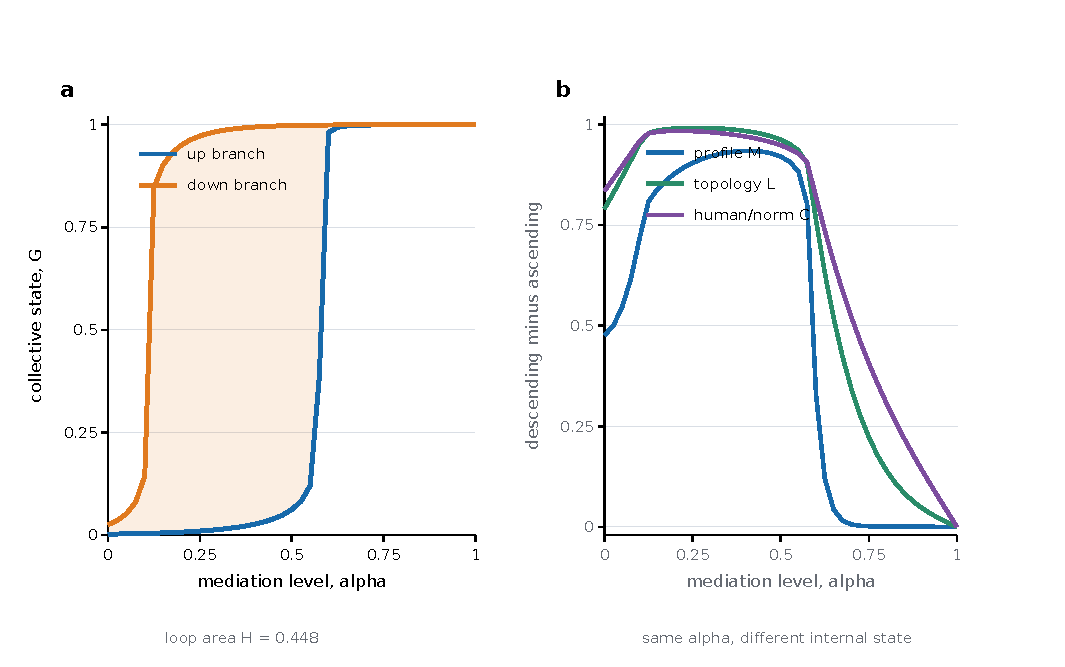
\includegraphics[width=\textwidth]{Fig3.pdf}
\caption{Baseline closed-loop simulation. (a) Ascending and descending branches at the same current mediation level. The shaded region is the signed loop area. (b) Down-minus-up differences in the three memory reservoirs.}
\label{fig:loop}
\alttext{Two panels show a large separation between ascending and descending collective-state curves at matched mediation and positive retained recommender, topology, and human-memory gaps on the return branch.}
\end{figure}

\subsection{Rate diagnostics remain nonzero over the tested range}

Within the known equations of Model I, loop area initially increases as the system has time to build slow memory and then declines as the return branch has more time to recover. This mechanism interpretation follows from the specified model; the same finite-rate pattern would not by itself exclude an arbitrarily slow monostable alternative in data. Across the tested range, the area remains $0.334$ at the slowest dwell, whereas the all-channel-ablated area is $0.013$ at the baseline dwell (Figure~\ref{fig:diagnostics}A). The constructed model combines rapid dynamic lag, memory accumulation, slow recovery, and a bistable fast landscape.

Rate variation distinguishes finite-speed signatures but cannot, over a finite range, rule out arbitrarily slow relaxation. A still slower ramp could eventually close the loop if all reservoirs are ergodic. Conversely, real platforms may never reach quasi-static equilibrium because content supply, events, and populations change. The empirical target is therefore rate-robust path dependence on societally relevant timescales, with explicit extrapolation uncertainty, not metaphysical proof of permanent irreversibility.

\subsection{Mechanism ablation is not state restoration}

For Model I, the original eight-cell diagnostic uses the scalar path deficit
\begin{equation}
D(R)=D_{\mathrm{path}}(R;v)
=\int_0^{\alphamax}
\left|\Delta_G^{(v)}(\alpha\mid R)\right|\,\dd\alpha,
\end{equation}
with $w(\alpha)=1$. In every reported ablation condition, the archived branch gap is nonnegative up to numerical rounding; hence $D(R)=\mathcal H_G(R)$ for this calibration. This equality is a property of these trajectories, not a general identity between absolute deficit and signed area.

Removing only the contribution of $M$ leaves $D=0.424$; removing only $C$ leaves $0.330$; removing only $L$ leaves $0.278$ (Figure~\ref{fig:diagnostics}B). Pairwise ablations reduce the deficit to $0.172$--$0.251$, and ablating all three contributions reduces it to $0.013$. These are whole-path mechanism ablations: they alter the equations before history is created. They neither restore a realized state at a reversal time nor solve Eq.~\eqref{eq:minimum-reversal-bundle}.

The M\"obius transform in Eq.~\eqref{eq:mobius} can still summarize non-additivity of this ablation lattice, but it must not be interpreted as a causal reset decomposition. Its pairwise coefficients are $0.078$ for $M$--$L$, $0.055$ for $M$--$C$, and $-0.012$ for $L$--$C$, with a three-way coefficient of $0.003$. The calculation is useful for generating intervention hypotheses; the corresponding restoration policies require their own time-indexed randomization.

\begin{figure}[!htbp]
\centering
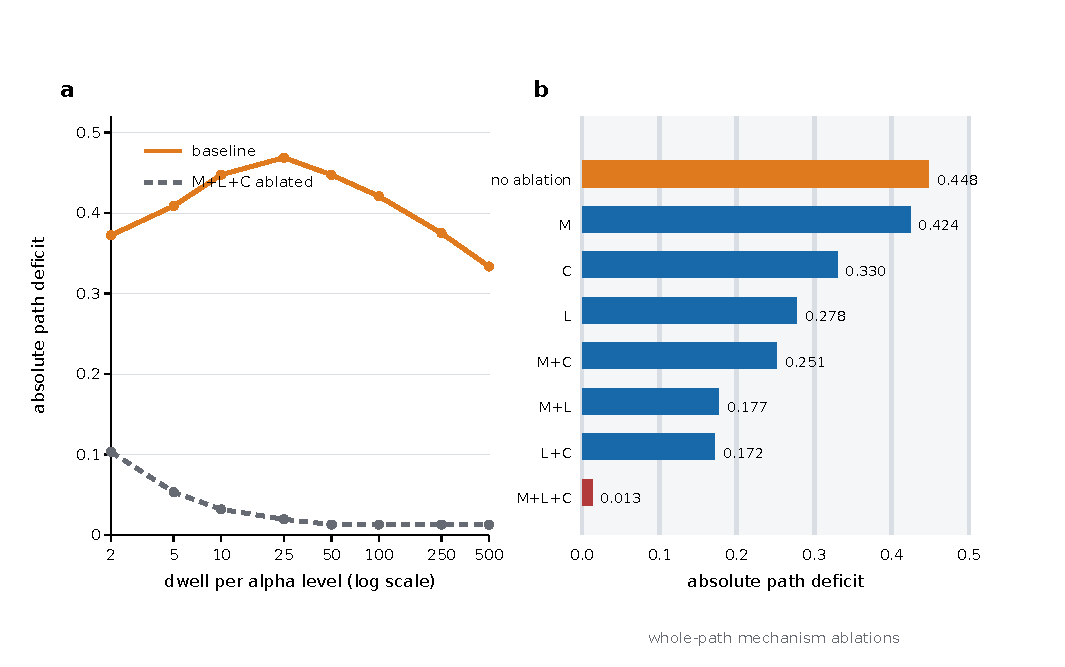
\includegraphics[width=\textwidth]{Fig4.pdf}
\caption{Rate and ablation diagnostics. (a) Loop area across dwell time for the constructed baseline and the model with all memory contributions removed. (b) Path deficit under the eight whole-path mechanism-ablation combinations. These operations modify the equations throughout the cycle; they are not state resets.}
\label{fig:diagnostics}
\alttext{The first panel shows a nonmonotone loop area that remains large at the slowest tested rate, unlike the all-channel-ablated model. The second panel compares all combinations of three whole-path mechanism ablations.}
\end{figure}

\subsection{Structural stress tests and time-indexed reversal policies}

The baseline parameterization lies in the bistable regime by construction; robustness is therefore assessed through structurally distinct parameterizations rather than local perturbations alone (Figure~\ref{fig:stress}). Crucially, a frozen-$M,L,C$ fold label does not classify the coupled system. At fixed $\alpha$, the three reservoir equilibria can be eliminated exactly:
\begin{equation}
\begin{aligned}
M^*&=\frac{\alpha G}{\alpha+\delta_M(1-\alpha)},\\
L^*&=\frac{(b_0+b_\alpha\alpha)G}{(b_0+b_\alpha\alpha)G+d_L(1-G)},\\
C^*&=\frac{\lambda_+G}{\lambda_+G+\lambda_-(1-G)}.
\end{aligned}
\label{eq:reservoir-equilibria}
\end{equation}
Substitution into Eq.~\eqref{eq:g} reduces every full equilibrium to one scalar root in $G$. We perform an equilibrium/stability scan on 401 $\alpha$ values using 20,001 $G$ points and classify every root with the exact full $4\times4$ Jacobian. Sign-change brackets are bisected for 70 iterations. Analytic stationary points supplement those brackets and are retained as tangential roots when the reduced residual is below $\epsilon_{\mathrm{root}}=10^{-9}$; near-grid roots use $10^{-10}$ and roots within $2\times10^{-5}$ are deduplicated. Stability requires $\max\Re\lambda<-\epsilon_\lambda$ with $\epsilon_\lambda=10^{-7}$. An independent 201-by-10,001 audit returns the same regime labels; transition locations are reported as finite grid brackets rather than pseudo-arclength continuation estimates. Appendix Table~\ref{tab:model-i-regime-parameters} gives every regime-specific override.

\begin{table}[!htbp]
\centering
\caption{Full-system classification of the five Model-I rate regimes. ``Fast'' describes only the frozen-reservoir $G$ subsystem; the classification uses all four coupled states.}
\label{tab:full-classification}
\small
\begin{tabularx}{\textwidth}{|p{3.7cm}|p{2.6cm}|p{2.8cm}|Y|}
\hline
\textbf{Parameterization used in Figure~\ref{fig:stress}A} & \textbf{Full-system class} & \textbf{Sampled multistable $\alpha$ interval} & \textbf{Smallest sampled stable margin $-\max\Re\lambda$}\\
\hline
Fast monostable, no memory & Monostable & None & $7.53\times10^{-4}$\\
\hline
Fast monostable + slow memory & Multistable & $[0.2925,0.4675]$ & $8.3\times10^{-5}$\\
\hline
Near-critical fast + memory & Multistable & $[0.2025,0.4500]$ & $2.25\times10^{-4}$\\
\hline
Bistable fast, no memory & Multistable & $[0.6500,0.6675]$ & $7.53\times10^{-4}$\\
\hline
Bistable fast + memory & Multistable & $[0.1525,0.4425]$ & $2.15\times10^{-4}$\\
\hline
\end{tabularx}
\end{table}

Only the first regime is monostable as a full system: its absolute area falls from $0.0072$ at dwell 5 to less than $10^{-12}$ by dwell 80. Adding slow reservoirs to the frozen-fast-monostable case changes the equilibrium geometry itself: the full system is multistable, with area $0.406$ at dwell 20 and $0.274$ at dwell 320. The near-critical-with-memory, memory-free bistable, and baseline regimes are also full-system multistable, with the intervals shown above. Their rate curves provide qualitatively different finite-speed signatures, but they do not uniquely identify the underlying mechanism or by themselves decompose finite-speed lag, slow memory, and multistability. That decomposition is why the empirical framework requires both the class-relative envelope and interventions.

\begin{figure}[!htbp]
\centering
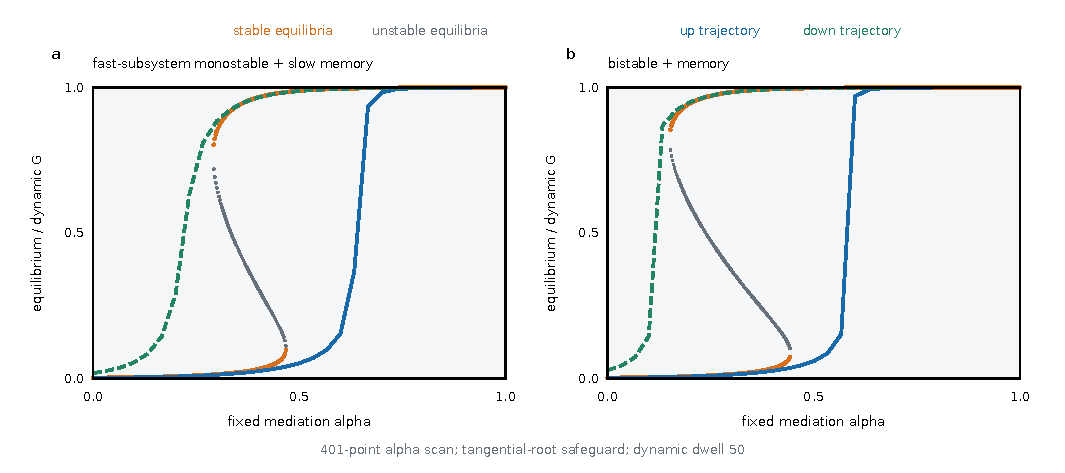
\includegraphics[width=\textwidth]{Fig6.pdf}
\caption{Grid-resolved fixed-alpha equilibrium geometry and finite-rate trajectories for two Model-I regimes. Stable and unstable full-system equilibria are classified by the exact four-state Jacobian; solid and dashed trajectories show the up and down branches at dwell 50. The derivative-based tangency safeguard and doubled-resolution audit prevent sign-change bracketing from hiding a sampled double root.}
\label{fig:bifurcation}
\alttext{Two panels overlay stable and unstable equilibrium branches with finite-rate ascending and descending trajectories. The slow-memory regime has multiple full-system equilibria despite a monostable frozen fast subsystem.}
\end{figure}

The loop is also present with a slope-matched probit response and under process noise across 64 independent seeds per link. This is structural stress, not calibration: an alternative sigmoid does not address heterogeneity, endogenous content supply, strategic objectives, or multidimensional beliefs. Separately, the archived 400-draw $\pm20\%$ experiment remains a local sensitivity analysis; its baseline 5th, 50th, and 95th area percentiles are $0.351$, $0.466$, and $0.610$. When the excluded topology rates are restored to the audit, 1,000 all-parameter Latin-hypercube draws give area percentiles $(0.345,0.438,0.574)$, reference-state-deficit percentiles $(0.467,0.642,0.842)$, and threshold-width percentiles $(0.40,0.50,0.65)$; all 1,000 retain a coarse multistability indicator. An independently coded adaptive Dormand--Prince 5(4) integrator reproduces the Euler level-end states for dwell 50 and 320 with maximum coordinate discrepancy $8.7\times10^{-4}$ and maximum $G$ discrepancy $1.1\times10^{-4}$.

A state intervention is applied after the turning-point observation and before the first descending dwell. The one-shot assignment $M,L\leftarrow0$ is labeled \emph{diagnostic zeroing}, not restoration: because $b_0>0$, the low-mediation reference generally has $L>0$. Zeroing has almost no effect because the reservoirs regenerate, with $D_{\mathrm{path}}=0.447$ versus $0.448$ without intervention. The reference-emulating policy instead assigns $M,L$ to their same-time values in the separately simulated stationary $\alpha=0$ control at the start of the descending branch. After every Euler update on the entire descending branch, both coordinates are clamped to that reference trajectory's next same-elapsed-time value. It reduces path deficit to $0.120$ and endpoint-state deficit from $0.656$ to $0.278$. Human-recovery facilitation acts only on the descending branch and multiplies $\lambda_-$ by four, from $0.045$ to $0.18$; alone it leaves path deficit $0.445$. Combining recovery with reference-emulating $M,L$ restoration reduces path and state deficits to $0.094$ and $0.051$. The example makes regeneration and reference fidelity part of the estimand and keeps human recovery semantically separate from platform-state restoration.

\begin{figure}[!htbp]
\centering
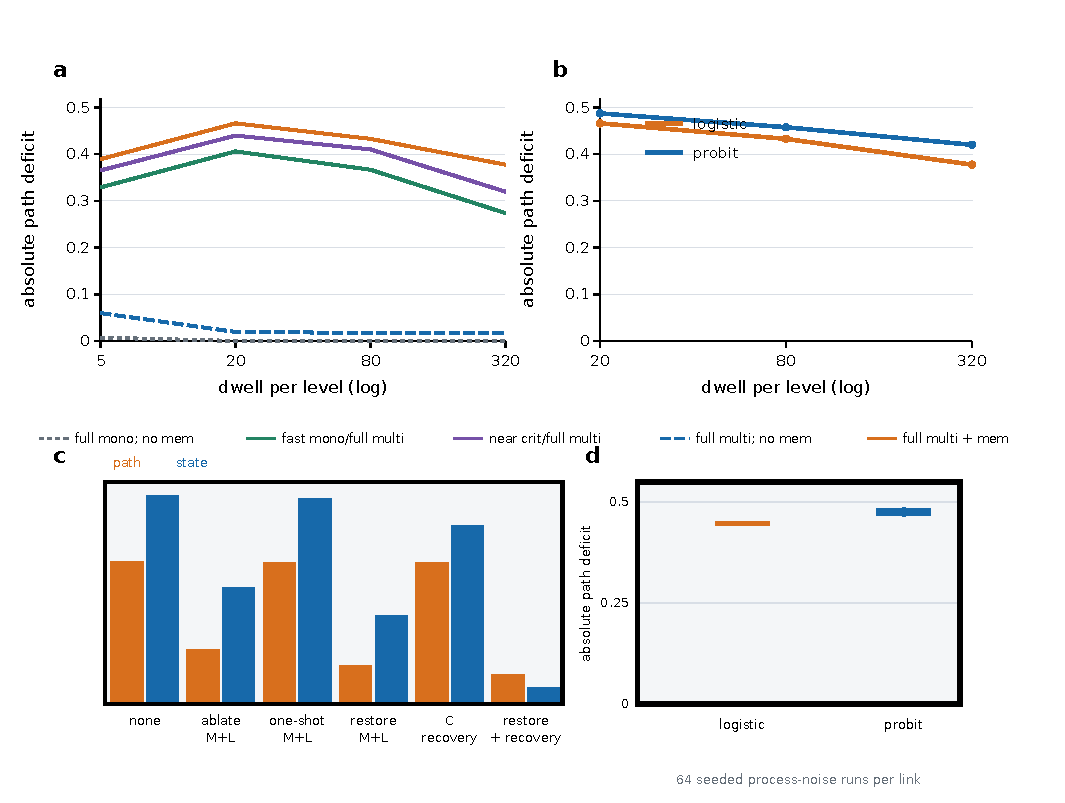
\includegraphics[width=\textwidth]{Fig5.pdf}
\caption{Structural and intervention stress tests for Model I. (a) Absolute path deficit across dwell times; legend labels distinguish the frozen-fast-subsystem descriptor from the full-system equilibrium/stability class in Table~\ref{tab:full-classification}. (b) Logistic and slope-matched probit links. (c) Path and endpoint-state deficits under whole-path ablation, diagnostic zeroing, reference-emulating restoration, and human-recovery facilitation. (d) Seed distributions under process noise.}
\label{fig:stress}
\alttext{Four panels compare rate responses across structural regimes, logistic and probit links, distinct intervention semantics, and stochastic seed distributions. A one-shot reset regenerates, whereas platform restoration plus human recovery most strongly reduces both deficits.}
\end{figure}

\section{Model II: an explicit adaptive network}

The scalar $L$ in Model I is a mean-field ledger entry, not a substitute for a graph. We therefore construct a second, deliberately minimal mechanism model in which node states and ties coevolve. Let $A_{ij}(t)=A_{ji}(t)\in\{0,1\}$, $A_{ii}=0$, denote an undirected social graph, let $x_i(t)\in[-1,1]$ be a continuous expressed state, and let the fixed label $s_i\in\{-1,+1\}$ identify one of two initially mixed camps. With $k_i=\sum_jA_{ij}$, the chronological social signal and ranked signal are
\begin{align}
u_i^{\mathrm{chr}}(t)
 &=\omega\frac{\sum_jA_{ij}(t)x_j(t)}{k_i(t)}
 +(1-\omega)a s_i,\\
u_i^{\mathrm{rank}}(t)
 &=\zeta\tanh\{\beta x_i(t)+\gamma s_i\}.
\end{align}
One synchronous update is
\begin{equation}
\begin{aligned}
x_i(t+1)
&=\operatorname{clip}_{[-1,1]}\Bigl[x_i(t)
 +\mu\bigl\{(1-\alpha)u_i^{\mathrm{chr}}(t)\\
&\hspace{4.8em}+\alpha u_i^{\mathrm{rank}}(t)-x_i(t)\bigr\}
 +\epsilon_{it}\Bigr],\\
\epsilon_{it}&\overset{\mathrm{iid}}{\sim}\mathcal N(0,\sigma_x^2),
\qquad \sigma_x=0.0035.
\end{aligned}
\label{eq:network-opinion}
\end{equation}
Noise is independent over nodes and updates and is added before the final projection. A dedicated opinion-noise stream is shared across paired regimes within each initialization; rewiring proposals use a separate stream, so a differing number of swaps cannot shift later opinion innovations. The learned ranker is represented only through its exposure target; it is not claimed to reproduce a production recommender. Rewiring is stochastic and degree preserving. Above a prespecified onset $\alpha_0$, two cross-camp edges are swapped into two within-camp edges. Below $\alpha_0$, the reverse operation swaps one within-camp edge from each camp into two cross-camp edges, up to the initial cross-edge count. Per update, attempted event counts are Poisson with means
\begin{equation}
N\rho_+\frac{(\alpha-\alpha_0)_+}{1-\alpha_0}
\quad\text{and}\quad
N\rho_-\frac{(\alpha_0-\alpha)_+}{\alpha_0},
\label{eq:rewiring-intensity}
\end{equation}
respectively. Reverse mixing restores a coarse structural target, not the identities of initial edges. The boundary case $\rho_-=0$ is retained explicitly as an irreversible stress condition rather than treated as the default mechanism.

The rewiring rule yields a network-specific reversal law before simulation. Let $B_t=|E_\times(t)|$, let $N_t^+$ and $N_t^-$ be the Poisson attempt counts in Eq.~\eqref{eq:rewiring-intensity}, and let $S_t^+\leq N_t^+$ and $S_t^-\leq N_t^-$ be accepted homophilic and reverse swaps after feasibility and cap checks.
\begin{proposition}[Bridge-count drift and finite-horizon repair]
\label{prop:bridge-drift}
Conditional on the pre-update graph $\mathcal F_t$ and current $\alpha$,
\begin{equation}
\E(B_{t+1}-B_t\mid\mathcal F_t,\alpha)
=2\{\E(S_t^-\mid\mathcal F_t,\alpha)-\E(S_t^+\mid\mathcal F_t,\alpha)\}.
\label{eq:bridge-drift}
\end{equation}
Away from graphical boundaries, if every attempted swap is feasible and the initial-bridge cap is inactive, this becomes
\begin{equation}
2N\left[\rho_-\frac{(\alpha_0-\alpha)_+}{\alpha_0}
-\rho_+\frac{(\alpha-\alpha_0)_+}{1-\alpha_0}\right].
\label{eq:interior-bridge-drift}
\end{equation}
On a fixed low branch $\alpha<\alpha_0$, write
\begin{equation}
\lambda_-(\alpha)=N\rho_-\frac{\alpha_0-\alpha}{\alpha_0},
\qquad k_t=\frac{\mathcal D_t}{2}\in\mathbb N,
\end{equation}
where $\mathcal D_t=B_0-B_t$. The quantity is even because every accepted swap changes $B$ by two and the dynamics preserve the parity of $B_0-B_t$. Under perfect feasibility, the number of reverse events in an integer horizon of $T$ updates is $N^-_{t:t+T}\sim\operatorname{Poisson}\{\lambda_-(\alpha)T\}$ and
\begin{equation}
\Pr(T_{\mathrm{repair}}\leq T)
=\Pr[\operatorname{Poisson}\{\lambda_-(\alpha)T\}\geq k_t].
\label{eq:reverse-budget}
\end{equation}
The ideal discrete repair time satisfies
\begin{equation}
\E(T_{\mathrm{repair}}^{\mathrm{ideal}})
=\sum_{n=0}^{\infty}
\Pr[\operatorname{Poisson}\{\lambda_-(\alpha)n\}<k_t].
\label{eq:ideal-mean-repair-time}
\end{equation}
Proposal infeasibility can only reduce the actual repair probability relative to the ideal tail and delay repair, so
\begin{equation}
\E(T_{\mathrm{repair}})
\geq \E(T_{\mathrm{repair}}^{\mathrm{ideal}})
\geq \frac{k_t}{\lambda_-(\alpha)},
\label{eq:mean-repair-time}
\end{equation}
where the second inequality is generally strict. The cap cannot delay first hitting of $B_0$: parity prevents an overshoot from below, and the cap only prevents moves beyond the restored target. If $\rho_-=0$, every deficit created by accepted homophilic swaps is absorbing under the stated topology rule.
\end{proposition}

Each accepted homophilic swap removes exactly two cross edges and each accepted reverse swap adds exactly two, proving Eq.~\eqref{eq:bridge-drift}; Poisson superposition yields Eq.~\eqref{eq:reverse-budget}. In a continuous-time Poisson embedding, the $k_t$th event time $S_{k_t}$ is Erlang with mean $k_t/\lambda_-$. Because the network is observed only at integer update boundaries, $T_{\mathrm{repair}}^{\mathrm{ideal}}=\lceil S_{k_t}\rceil$, which gives Eq.~\eqref{eq:ideal-mean-repair-time} by the tail-sum formula and implies $\E(T_{\mathrm{repair}}^{\mathrm{ideal}})\geq k_t/\lambda_-$, generally strictly. Proposal infeasibility can only delay repair; the initial-bridge cap prevents movement above, rather than first arrival at, the parity-compatible target. Unlike an exponential relaxation ansatz, the constant-rate rule predicts approximately linear bridge recovery until the cap. The simulation retains all boundary failures and reports observed drift and proposal acceptance against the interior prediction.

We track four states. For the fixed camp partition, let $m$ be the number of edges, $m_c$ the number of within-camp edges in camp $c$, $e_c=m_c/m$, $a_c=\operatorname{vol}(c)/(2m)$, $E_\times$ the cross-camp edge set, and $\operatorname{vol}(c)=\sum_{i:s_i=c}k_i$.
\begin{table}[!htbp]
\centering
\caption{Adaptive-network observables and their memory interpretation.}
\label{tab:network-metrics}
\small
\begin{tabularx}{\textwidth}{|p{1.2cm}|p{4.1cm}|Y|}
\hline
\textbf{Metric} & \textbf{Definition} & \textbf{Interpretation}\\
\hline
$Q$ & $\sum_c(e_c-a_c^2)$ for the fixed two-camp partition & Newman--Girvan modularity; higher values indicate stronger topological segregation\\
\hline
$r_x$ & $\operatorname{corr}(x_i,x_j)$ over both orientations of every edge & Opinion assortativity of connected nodes; depends jointly on $A$ and $\bm x$\\
\hline
$\phi$ & $|E_\times|/\min_c\operatorname{vol}(c)$ & Cross-camp conductance; lower values indicate a weaker bridge cut\\
\hline
$P$ & $N^{-1}\sum_i|x_i|$ & Mean absolute expressed state; a node-level polarization summary rather than a second cut metric\\
\hline
\end{tabularx}
\end{table}

\begin{table}[!htbp]
\centering
\caption{Complete Model-II parameterization. Rates $\rho_\pm$ are varied by regime; every other quantity is fixed before comparing paths.}
\label{tab:model-ii-parameters}
\small
\begin{tabularx}{\textwidth}{|p{2.6cm}|p{2.0cm}|Y|}
\hline
\textbf{Quantity} & \textbf{Value} & \textbf{Role}\\
\hline
$N,m$ & $80,240$ & Nodes and undirected edges; the complete degree sequence is preserved\\
\hline
Initial cross-edge target & $B_0=96=0.40m$ & Exact bridge count before the chronological burn-in\\
\hline
Camp construction & balanced $\{-1,+1\}$ & Fixed labels with a connected Hamiltonian-cycle seed graph\\
\hline
Pre-burn-in opinions & $0.16s_i+\eta_i-\bar\eta$; $\sigma_0=0.022$ & Centered iid Gaussian innovations, projected to $[-1,1]$ before burn-in\\
\hline
Burn-in; path grid & $120$; $21+20$ blocks & Chronological equilibration; ascending and descending levels\\
\hline
Dwell & $30$ or $120$ updates & Baseline and four-times-slower path\\
\hline
$\mu,a,\omega$ & $0.13,0.18,0.82$ & Opinion step, identity anchor, chronological social weight\\
\hline
$\zeta,\beta,\gamma$ & $0.94,2.40,0.72$ & Ranked-target extremity, self-state weight, camp weight\\
\hline
$\alpha_0$; reset level & $0.50;0.50$ & Rewiring onset and descending graph-restoration point\\
\hline
$(\rho_+,\rho_-)$ & $(0,0)$; $(.010,.020)$; $(.010,.0025)$; $(.010,0)$ & No rewiring; fast reverse mixing; slow reverse mixing; one-way boundary\\
\hline
Opinion innovation & $\mathcal N(0,0.0035^2)$ & Independent node noise after each experimental-path opinion update; zero during burn-in\\
\hline
Initializations & $32$ & Seeds 20270824--20270855; common start across regimes within seed\\
\hline
Proposal limits & $96$ homophilic; $128$ reverse & Maximum candidate-pair trials per attempted degree-preserving swap\\
\hline
\end{tabularx}
\end{table}

The stress test uses the complete parameterization in Table~\ref{tab:model-ii-parameters}. Within a seed, every regime starts from the same graph and node state. The initializer asserts both $|E|=240$ and the exact cross-edge target $|E_\times|=96$. The Hamiltonian-cycle seed guarantees $k_i\geq2$, and degree preservation maintains this bound, so the denominator of $u_i^{\mathrm{chr}}$ never vanishes. The turning-point observation is shared on the 21-point matched grid. We cross no rewiring; fast reversible rewiring; slow reverse mixing; four-times-slower ramps; the one-way boundary; and a graph restoration $A\leftarrow A(0)$ at descending $\alpha=0.5$ while retaining $\bm x$. Model II has no content-production or recommender-learning layer: its only theoretical role is to realize the topological reservoir and test the finite-horizon bridge prediction.

For $(Q,r_x,\phi,P)$, the no-rewiring control has median areas $(0,0.0065,0,0.0046)$. Fast reversible rewiring yields
\begin{equation}
(0.128,0.228,0.132,0.096),
\end{equation}
which contracts to $(0.055,0.101,0.057,0.043)$ when dwell rises from 30 to 120. Slow reverse mixing gives $(0.219,0.364,0.228,0.165)$ and contracts under the slower ramp to
\begin{equation}
(0.106,0.177,0.109,0.082).
\end{equation}
The one-way boundary is strongest, at $(0.273,0.435,0.283,0.226)$ with large nonzero endpoint gaps. Across 32 initializations, the irreversible $\rho_-=0$ regime produces substantially larger loop areas than either reversible regime. It should therefore be interpreted as a boundary condition, not as representative behavior of the reversible model.

Graph restoration under slow reverse mixing reduces the $(Q,r_x,\phi,P)$ median areas to
\begin{equation}
(0.066,0.120,0.068,0.045).
\end{equation}
The complete median endpoint-gap vector $(Q,r_x,\phi,P)$ is $(0,0.028,0,0.0040)$. Thus exact adjacency restoration need not restore the joint state $(A,\bm x)$. This is a synthetic instance of false closure, not evidence about a platform.

The bridge-drift audit distinguishes the interior law from its feasibility envelope. Across the 30 regime--level blocks in which the relevant swap acceptance rate is at least $0.95$, observed and predicted drift have correlation $0.998$ and mean absolute error $0.018$ cross edges per update. Across all 180 nonzero-prediction blocks, boundary failures and the cap reduce that correlation to $0.254$. Figure~\ref{fig:bridge-validation} confirms the interior drift law when proposal feasibility is high and quantifies its breakdown when graphical constraints and the bridge cap bind.

\begin{figure}[!htbp]
\centering
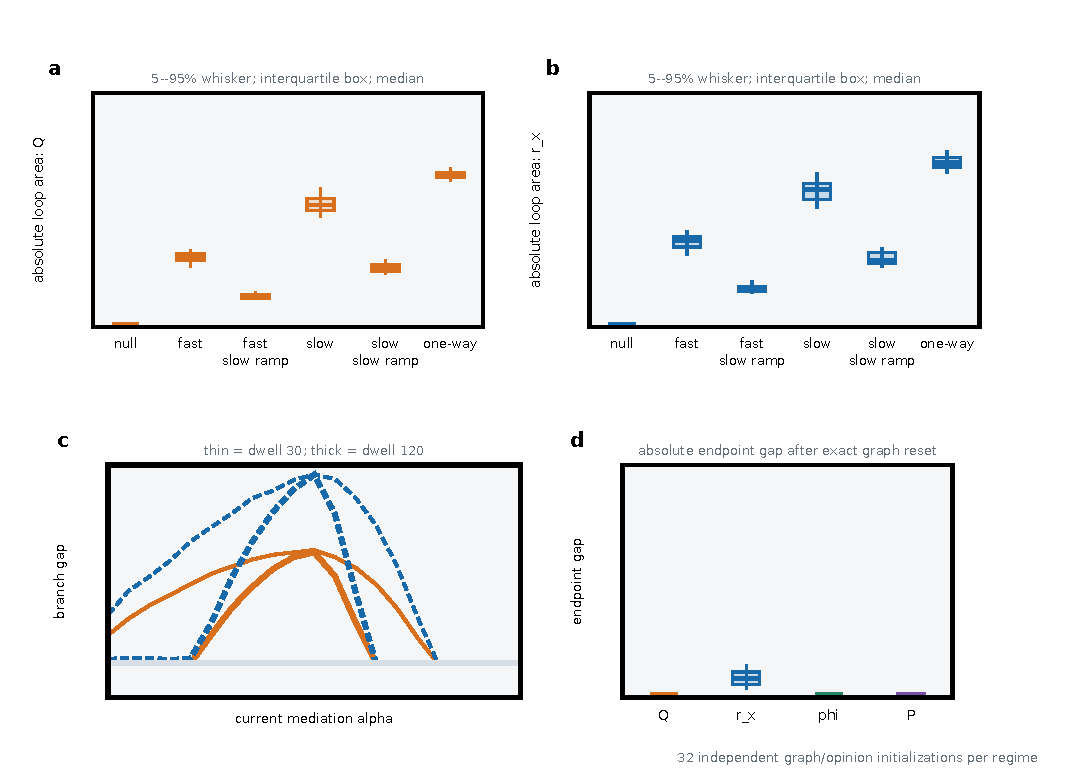
\includegraphics[width=\textwidth]{Fig7.pdf}
\caption{Adaptive-network stress test across 32 independent initializations. Panels report absolute loop area for modularity $Q$, opinion assortativity $r_x$, conductance $\phi$, and mean absolute opinion $P$. Reversible regimes are compared across rates; the one-way rule is an explicit boundary; and topology restoration resets $A$ while retaining $\bm x$. Points are seed-level values and bars summarize their distributions.}
\label{fig:adaptive}
\alttext{Four panels show seed distributions of loop areas across no-rewiring, reversible, slow-ramp, one-way-boundary, and graph-restoration regimes. Slower ramps contract reversible loops, while the one-way boundary produces the largest persistence.}
\end{figure}

\begin{figure}[!htbp]
\centering
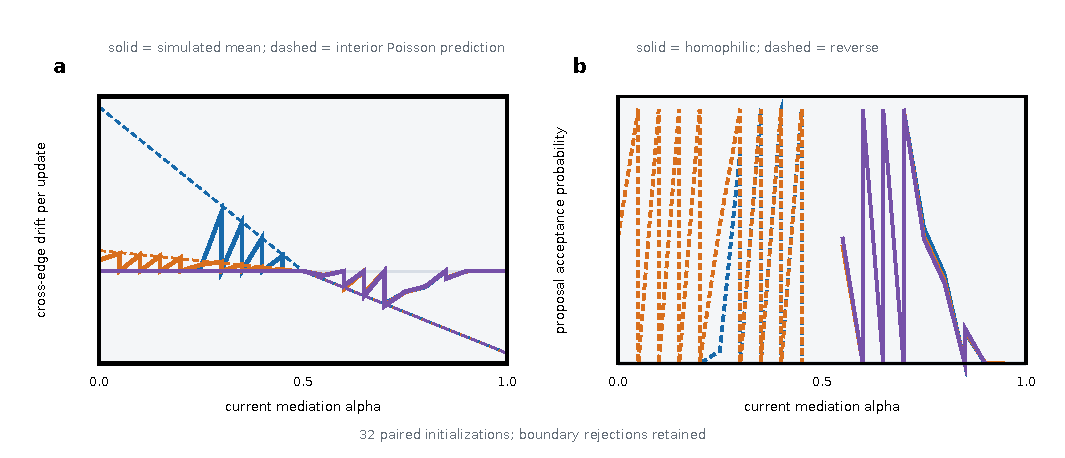
\includegraphics[width=\textwidth]{Fig8.pdf}
\caption{Finite-horizon validation of Proposition~\ref{prop:bridge-drift}. The left panel compares the observed block-level bridge update with the ideal interior drift, while the right panel reports accepted/proposed swap rates. Deviations are not simulation error: they expose graphical infeasibility and the initial-bridge cap that turn the interior formula into an upper repair budget.}
\label{fig:bridge-validation}
\alttext{Two panels compare observed and ideal cross-edge changes and show swap acceptance rates. Agreement is close in the interior, whereas boundary and cap regimes display lower observed repair than the unconstrained prediction.}
\end{figure}

Model II introduces an explicit adaptive topology while remaining deliberately stylized: camps are fixed, content production and recommender learning are absent, and $Q$ and $\phi$ are dependent summaries of the same planted cut. The independent $P$ summary and multi-seed stochastic design prevent four correlated cut metrics or one initialization from masquerading as four replications. The adaptive-network experiment establishes two model-level results: a topological reservoir can generate finite-rate branch dependence under reversible rewiring, and the persistence of that dependence is controlled by reverse-mixing capacity and graphical feasibility. These are mechanism results, not platform-level empirical estimates.

\section{A causal experiment for algorithmically mediated social hysteresis}

\subsection{Two implementation tiers}

\inlinehead{Tier 1: controlled experimental micro-platform.} The first implementation is a purpose-built, low-stakes social environment in which candidate-generation rules, ranking interpolation, profile state, link recommendations, interface, and restoration fidelity are under experimental control. Its limited scale constrains external validity, but permits repeated rates, minor loops, and direct mechanism measurement. The platform-state experiment randomizes technically realizable $M/L$ policies. A $C$ intervention is analyzed in a separate recovery trial as a non-coercive washout, norm correction, or deliberative experience---never literal erasure of a participant's belief.

\inlinehead{Tier 2: platform-scale field experiment.} A platform partnership adds natural social stakes, a mature recommender, and large-network interference. It requires version-locked ranking, a common candidate-generation \emph{rule}, auditable restoration, staggered cohorts, and measurement of cross-cluster exposure. Realized candidate sets are allowed to evolve in the primary total-system estimand. This tier may support only a subset of the platform-state intervention lattice; localization claims are restricted to channels with defensible fidelity, stability, and exclusion.

\subsection{Treatment and experimental unit}

The treatment must be manipulable, interpretable, and stable. Let $\alpha$ be the fraction of eligible impressions selected by a fixed version of a learned ranker, with the remainder selected by a preregistered chronological or followed-account rule. Candidate-generation rules, moderation, advertising load, and interface are held fixed; realized candidates need not be equal across histories. Equality of $\alpha$ alone is therefore called matched current policy only when these versioned components and the exposure mapping also match. A candidate-standardization substudy instead samples from the history-blind, common-support law $\Lambda$ defined above and answers the different question in Eq.~\eqref{eq:total-system-effect}.

Naive individual randomization is generally insufficient when interference is material. The preferred unit is a network cluster with low measured between-cluster exposure. Clusters are randomized to ordered sequences and ramp rates. The primary partial-interference design uses graph-separated clusters and reports cross-cluster impressions. If separation is infeasible, a two-stage saturation design first randomizes cluster-level history saturation and then individual assignment, estimating direct and exposure-policy effects. Both analyses use a preregistered exposure mapping and sensitivity curves for mapping violations; inference under the saturation design must reassign at the level of the actual two-stage allocation rather than recycle a no-interference test \cite{hudgens2008interference,aronow2017interference,liu2026saturation}.

\subsection{A gatekept experimental program}

The complete framework is too expensive and multiplicity-prone for one omnibus experiment. Figure~\ref{fig:design} therefore defines five gates. Stage 0 is a blinded pilot used to lock compliance, variance, intracluster correlation, leakage, attrition, and the measurement scale; independent stationary arms and prior engineering evidence define the candidate relaxation class without using branch outcomes to tighten it. Stage 1 randomizes mirrored up--down and down--up paths, with stationary low- and high-$\alpha$ controls and staggered cohorts. Stage 1 passes only when the preregistered simultaneous weak-null test rejects a zero average complete-history branch vector; Fisher's exact sharp-null test is a labeled companion analysis, not the gate. Stage 2 additionally requires that the externally justified class produce a nonvacuous envelope at feasible rates; otherwise the study stops at a design-based history-effect claim. Fresh Stage-2 clusters receive the locked multiple rates. Stage 3 randomizes factorial $M/L$ platform-restoration policies, including one-shot and regeneration-blocking versions. Human-recovery facilitation is a separate welfare-governed module. Stage 4 tests minor loops, new maxima, and replication.

Switchback theory informs spacing and inference under serial correlation \cite{bojinov2023switchback}. Unlike a conventional crossover, branch-specific carryover is the object of interest; calendar drift, ordinary adaptation, and cross-cluster exposure are threats. Carryover and dynamic-effect methods clarify this distinction \cite{wang2024carryover,sun2025dynamic}. Each gate has a preregistered stopping decision, so a null Stage-1 result terminates the mechanism program rather than inviting post-hoc searches.

\begin{figure}[!htbp]
\centering
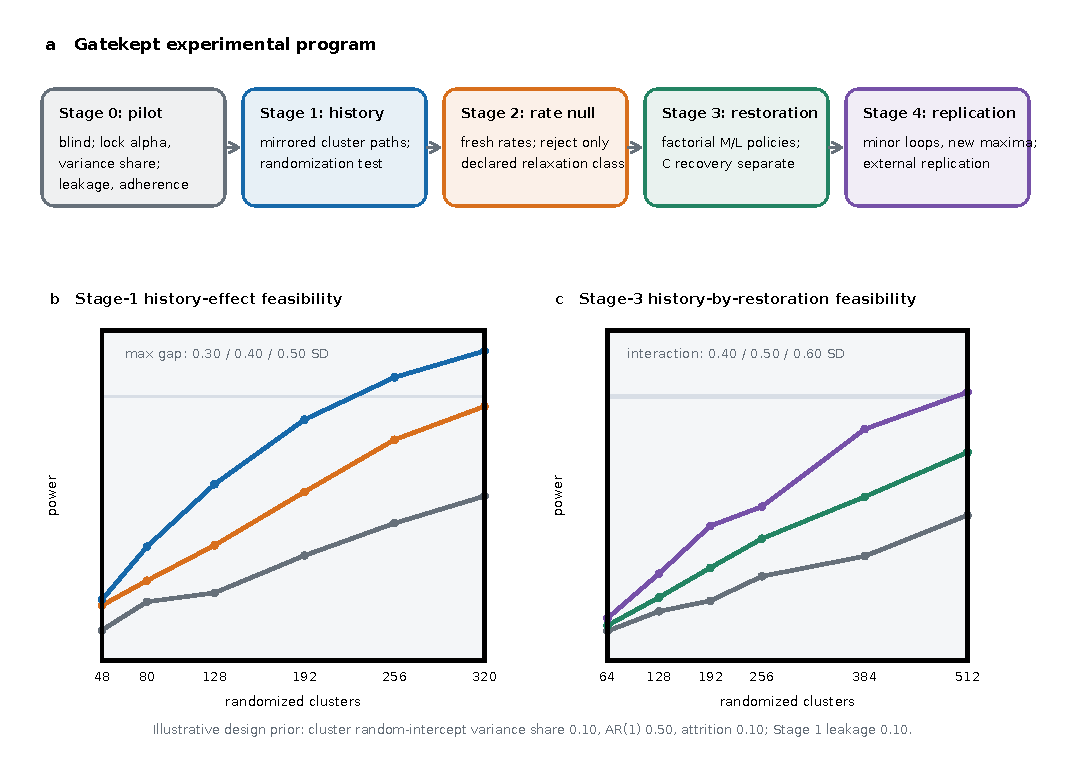
\includegraphics[width=\textwidth]{Fig9.pdf}
\caption{Gatekept experimental program and simulation-based feasibility screen. (a) Stages 0--4 separate history detection, relaxation-class testing, platform restoration, human recovery, and replication. (b,c) Power of studentized maximum statistics under an illustrative design prior; these curves are not a final sample-size determination.}
\label{fig:design}
\alttext{Five connected stage boxes show a blinded pilot, history test, rate-null test, restoration experiment, and replication. Two lower panels plot feasibility-screen power against randomized cluster count for several standardized history and history-by-restoration effects.}
\end{figure}

\subsection{Outcomes and mechanism measurements}

The primary outcome should not default to a single polarization index. A defensible preregistration specifies one primary construct and a small family of mechanism-resolving outcomes:
\begin{itemize}
  \item \textbf{Exposure:} ideological or topical assortativity, source diversity, cross-cutting conductance, and concentration;
  \item \textbf{Topology:} induced follows, unfollows, modularity, reciprocity, bridge persistence, and link-recommendation acceptance;
  \item \textbf{Behavior:} engagement, sharing, dwell, creation, and migration across communities;
  \item \textbf{Human state:} repeated attitudes, affective polarization, preference certainty, identity centrality, and perceived norms;
  \item \textbf{Algorithmic state:} score changes on a fixed candidate audit set, embedding drift, retained labels, and counterfactual rankings under frozen profiles.
\end{itemize}
The design separates exposure from attitude because algorithms can strongly change what is seen while leaving a rigid short-run attitude scale unchanged. The Facebook and Instagram studies make this distinction empirically essential \cite{guess2023feeds,nyhan2023likeminded,gonzalez2023segregation}. The X experiment additionally suggests that induced follows are a plausible topological mediator of branch asymmetry \cite{gauthier2026x}.

\subsection{Primary analysis}

The primary Stage-1 estimand is the vector of average complete-history branch contrasts over the prespecified interior grid. The maximum absolute studentized cluster-level difference is its multiplicity-controlled test statistic; a companion area statistic is secondary. Exact reassignment of complete cluster histories tests Fisher's sharp null that assignment changes no cluster-window outcome. Because that sharp null is stronger than the weak null of zero average branch contrast, the manuscript does not equate the two: average-effect point estimates and simultaneous intervals use a studentized cluster randomization procedure with weak-null-robust variance, while Fisher $p$-values are labeled sharp-null tests \cite{wu2021randomization}. This controls selection of the most favorable $\alpha$ without making the mixed model primary.

For descriptive smoothing and covariate precision, a preregistered generalized additive mixed model may estimate
\begin{align}
G_{cpt}
  &=\beta_0+f(\alpha_{cp})+I_{cp}^{\downarrow}g(\alpha_{cp}) \notag\\
  &\quad +f_v(v_c,\alpha_{cp})+\bm\gamma^\top\bm X_{c0}
  +u_c+\lambda_t+\varepsilon_{cpt}.
\end{align}
where $g(\alpha)$ is the branch contrast, $f_v$ is the rate interaction, $u_c$ is a cluster effect, and $\lambda_t$ absorbs calendar shocks. This model is secondary because misspecified smoothness or random-effects structure must not determine the primary claim.

Inference proceeds in three layers. First, the functional randomization analysis identifies a complete-history effect over the matched-current-policy interval. Second, if the prospective vacuity gate passes, fresh rate arms compare simultaneous lower confidence bounds on the absolute \emph{mean} branch gaps with the conservative step or continuous envelope in Eq.~\eqref{eq:lag-envelope}. This rejects only the externally declared class; a direct low-dimensional $W_1$ analysis is optional. Third, randomized restoration policies estimate $A_{J,j}$, $D_{\mathrm{path}}$, and $D_{\mathrm{state}}$; the full cost--deficit frontier is reported even when $\mathcal F_\epsilon$ is empty.

Mechanism analysis uses randomized mediator interventions where available; sequential g-computation is secondary and observational mediation is labeled exploratory. Generalized random forests may characterize preregistered treatment heterogeneity, but only after the average branch estimand is established \cite{athey2019forests}. Missingness, noncompliance, and attrition are analyzed by initial assignment, with inverse-probability sensitivity analyses and Lee-type bounds where assumptions are credible.

\subsection{Simulation-based feasibility screen}

Power must be evaluated for the randomization procedure actually used, not a cross-sectional $t$ test. The archived screen simulates one aggregate outcome per cluster and policy point, with a persistent cluster random-intercept variance share of $0.10$ across windows, AR(1) residual correlation $0.50$, attrition $0.10$, and, for Stage 1, cross-arm leakage $0.10$. This is not an individual-level intracluster correlation because the screen contains no within-cluster user outcomes. Every synthetic dataset receives a fresh balanced allocation, independent Bernoulli attrition, and a dataset-level reassignment distribution: the five-point studentized maximum is recomputed under each of 499 Monte Carlo reassignments. Each scenario uses 1,000 outer datasets. The corresponding Monte Carlo standard error is reported cell by cell and is at most $0.016$; the empirical type-I range across the displayed sharp-null designs is $0.041$--$0.056$. In the separate false-sharp/true-weak-null audit, exactly mean-zero heterogeneous effects yield rejection rates $0.049$, $0.035$, and $0.037$ as heterogeneity amplitude rises from $0.40$ to $1.20$. The screen is a feasibility calculation and implementation sanity check, not a tail-accurate final design or a proof of weak-null validity.

The feasibility screen shows that the proposed cluster-randomized design requires large sample sizes for moderate standardized branch effects. With the broad-hump shape, a maximum input gap of $0.50$ reaches power $0.858$ at 256 clusters, whereas a $0.40$ gap reaches $0.770$ at 320 clusters. The reported effects precede Stage-1 leakage attenuation. For the Stage-3 factorial, an interaction of $0.60$ reaches $0.813$ at 512 clusters; $0.50$ reaches $0.631$. These values establish feasibility constraints rather than a sample size. At a fixed representative design, changing the signal from a localized threshold to a broad plateau shifts power from $0.582$ to $0.837$ in Stage 1 and from $0.440$ to $0.691$ in Stage 3. A final calculation must lock nuisance ranges from Stage 0, incorporate unequal cluster sizes and the exact allocation, and use at least 20,000 outer datasets per candidate design. Appendix~\ref{app:power-dgp} gives the complete data-generating process.

\subsection{Falsification and alternative explanations}

A credible empirical case for hysteresis requires, at minimum, the following falsification tests:
\begin{enumerate}
  \item \textbf{Rate test:} the branch gap remains at slower ramps or follows an explicitly estimated rate law.
  \item \textbf{Stationary test:} at fixed $\alpha$, secular trends cannot reproduce the sign and shape of the branch interaction.
  \item \textbf{Calendar test:} the result replicates across staggered cohorts and non-overlapping event windows.
  \item \textbf{Candidate-standardization test:} a randomized $\Lambda$ substudy estimates $\tau^{K\text{-}\mathrm{ctrl}}$; its difference from the total-system effect is reported as an estimand contrast, not a balance correction.
  \item \textbf{Novelty test:} interface switching without ranking changes does not reproduce the loop.
  \item \textbf{Selection test:} initial feed preference and compliance do not explain apparent on/off asymmetry.
  \item \textbf{Minor-loop test:} partial reversals yield reproducible nested trajectories rather than arbitrary drift.
  \item \textbf{Negative-control test:} outcomes not plausibly affected by the ranker show no corresponding branch pattern.
\end{enumerate}

\subsection{Ethics and stopping rules}

The strongest experiment is not the one that maximizes a harmful state. The initial implementation should use low-stakes, non-clinical, non-electoral content with adult participants who understand that feed ordering is experimentally varied. The protocol requires independent review, data minimization, content risk screening, prespecified maximum exposure, participant-controlled exit, debriefing, and real-time stopping thresholds for distress, harassment, extremist exposure, or disproportionate group harm. No intervention should target protected traits, suppress lawful political viewpoints, or intentionally radicalize participants. A platform field experiment should publish treatment logic and an audit set sufficient for independent replication without exposing personal profiles.

\section{Framework-level tests and mechanism-specific hypotheses}

The framework itself makes three falsifiable commitments. First, a Stage-1 claim requires a randomized branch-law difference at matched current policy, not merely asymmetric pre/post coefficients. Second, a relaxation-class rejection claim requires the joint lower confidence limit to exceed a nonvacuous prespecified rate envelope; persistence over a convenient finite range is insufficient. Third, reversal controllability requires both path and endpoint-state tolerances under an admissible randomized policy. Failure at any gate stops the corresponding claim.

Minor-loop geometry is a framework-level diagnostic but has no predetermined sign: reproducible dependence on the previous maximum constrains memory, while exact return-point closure is not required. Platform heterogeneity is likewise an estimand, not a universal direction.

The following stronger hypotheses belong to Model I and must not be generalized by definition. Longer residence near $\alphamax$ initially increases reservoir loading and eventually saturates it. Profile and exposure differences precede topology and human/normative changes; on withdrawal, profile effects decay first unless retention is explicit. $M/L$ restoration has a larger effect when regeneration is blocked, and its interaction with $C$ recovery can be nonadditive. Model II adds the hypothesis that reversible topological loops contract as reverse-mixing time becomes short relative to the ramp, whereas the one-way boundary retains a nonzero structural endpoint gap.

These hypotheses are explicitly falsifiable: a well-powered null result rules out the corresponding mechanism at the tested scales, rates, and intervention fidelity. A failure of the stochastic envelope to be nonvacuous also narrows the framework more meaningfully than another one-shot on/off comparison.

\section{Implications for algorithm governance}

An on/off audit treats the algorithm as a contemporaneous treatment. A hysteresis audit treats the platform as a stateful intervention system. The distinction changes governance in four ways.

First, a right to disable personalization may reduce current ranking while leaving induced follows, creator supply, learned preferences, and perceived norms intact. The policy can be valuable without restoring the counterfactual pre-exposure state. Second, if path dependence is a material concern, impact assessment would need to record maxima, duration, and trajectories of exposure, not only the current setting. Third, the framework adds reversal cost as an evaluation target: the intervention cost required to return the system within prespecified path and state tolerances. Fourth, sunset clauses for ranking objectives could specify memory handling, including retention of inferred profiles and treatment of algorithmically induced ties.

The framework does not imply that diversity maximization is always beneficial. Exposure to opposing views can backfire \cite{bail2018opposing}, and normative-feed interventions can change perceptions through mechanisms that require context-specific evaluation \cite{brady2026norms}. Anti-hysteretic design therefore means controllable, measurable, and reversible mediation, not automatic counter-attitudinal content.

\section{Discussion}

The framework is built around a distinction that conventional withdrawal designs often leave implicit: current treatment does not determine current state. Once a recommender changes the topology and the people it mediates, the reverse switch answers a different causal question from the forward switch. The framework provides a testable explanation for asymmetric introduction and withdrawal effects: withdrawal can occur from a state that prior algorithmic exposure has already changed. A null effect of algorithm removal can therefore coexist with a substantial historical effect of algorithm introduction if prior exposure constructed pathways that remain in the nominal control feed. The 2026 X experiment reports persistent algorithm-induced follows, providing a concrete candidate state variable through which treatment history could affect later outcomes \cite{gauthier2026x}. It does not, however, identify a closed hysteresis loop.

The theoretical contribution is not the logistic fold condition, nor the premise that withdrawal can be asymmetric. Lemma~\ref{lem:finite-record-equivalence} shows why finite binary or graded records do not identify an unrestricted latent class; Proposition~\ref{prop:stochastic-rate-separation} supplies a falsifiable distributional boundary for a declared stochastic relaxation class; and Proposition~\ref{prop:reset-separation} states when a time-indexed restoration can separate histories. Together, the paired reversal deficit changes the question from ``is there a loop?'' to ``which state can be restored, by which admissible policy, at what cost and horizon?''

The two models serve different roles. Model I exposes a fold and three slow reservoirs in four equations, then demonstrates why ablation, one-shot reset, reset-and-freeze, and recovery are distinct operations. Model II shows that a topological reservoir can arise from bidirectional degree-preserving rewiring and that its apparent irreversibility depends strongly on reverse-mixing rate; exact graph restoration still need not restore node states. Neither synthetic model is empirical evidence. Richer models should challenge these mechanisms under multidimensional belief, endogenous content creation, strategic platforms, heterogeneous susceptibility, and cross-platform movement.

The proposal also reframes carryover. In pharmaceutical crossover designs, carryover can invalidate a treatment contrast. In the present design, branch-specific carryover is the object of interest, while calendar effects, ordinary adaptation, and uncontrolled exposure are threats. This does not eliminate the identification problem; it clarifies it. Multiple sequences, stationary arms, staggered entry, rate variation, and mechanism-specific resets are needed because a two-period crossover cannot separate all relevant histories.

Three conceptual limits deserve emphasis. First, $\alpha$ is an engineered control, not a natural scalar. Results do not transfer between platforms unless the intervention is mapped through exposure and ranking diagnostics. Second, hysteresis need not be harmful. Memory can stabilize prosocial norms, protect communities from transient shocks, or preserve trusted relations. The sign of $G$ and the welfare function are empirical and normative choices. Third, irreversibility is time-scale dependent. A loop may persist for months and vanish over years; that can still matter for elections, public health, or collective action without being permanent.

\section{Limitations}

The numerical results are synthetic and uncalibrated. The normal form compresses heterogeneous people, content, and networks into one order parameter; its baseline was selected just above a fold, not estimated from data. The structural stress tests cover five parameterizations whose full equilibria are classified on a dense equilibrium/stability grid with analytic tangency safeguards and a second-resolution audit, one slope-matched alternative link, and additive process noise, not the space of plausible social mechanisms. An independent adaptive Runge--Kutta implementation checks the Euler trajectories but does not prove solver-independence. The $\pm20\%$ experiment is local; the all-parameter Latin-hypercube analysis is still bounded to the declared hyperrectangle. The adaptive network uses 32 initializations but fixed camps, a planted cut, no content-production or recommender-learning layer, and only two dependent structural metrics plus two joint/node-state metrics. Proposition~\ref{prop:bridge-drift} predicts cross-edge drift only for the stated swap rule; feasibility failures make its interior expression optimistic. Exact platform-state restoration is idealized; human memory cannot ethically be reset.

The literature search is broad but not a formal systematic review. It used nine OpenAlex query families, backward chaining, DOI validation, and targeted additions through 26 August 2026. Database coverage, language, terminology, and indexing can omit relevant work. The paper therefore claims a structured audit across adjacent literatures, not literal exhaustiveness.

The proposed experiment is demanding. Tier 1 sacrifices external validity for control; Tier 2 requires platform cooperation. Network interference, candidate evolution, noncompliance, product updates, events, attrition, and strategic creator response can all produce branch-like patterns. The feasibility screen assumes equal cluster sizes and a stylized covariance model; 1,000 outer datasets and 499 reassignments per dataset are insufficient for a final tail-calibrated design. A finite rate collection cannot nonparametrically prove a quasistatic limit, and an unverified reset identifies only a policy interaction. Finally, social outcomes are multidimensional: no loop area is a welfare measure.

\section{Conclusion}

This paper provides a causal framework for testing whether the same current algorithmic policy produces different social outcomes because it was reached through different treatment histories. It separates that design-based history effect from stronger claims about quasistatic hysteresis and asks a second question that standard withdrawal studies leave unanswered: whether the state created by prior mediation can be restored. The first question has a precise experimental form:
\begin{equation}
0\rightarrow\alphamax\rightarrow0,
\qquad
\Gup(\alpha)\stackrel{?}{=}\Gdown(\alpha).
\end{equation}
Identifying a causal history effect requires randomized histories observed at matched current policy. Distinguishing that effect from ordinary finite-rate relaxation additionally requires rate variation and an explicit relaxation null. Determining where memory resides and whether it can be reversed requires state-resolving measurements and restoration interventions. The two models show how recommender profiles, induced topology, and human consolidation can make an off-switch causally incomplete. The proposed protocol turns those mechanisms into a falsifiable research program whose central output is an estimate of whether a mediated social state is reversal-controllable, how much reversal costs, and which memory paths must be interrupted. Restoring treatment is an operation. Restoring state is a causal achievement.

\section*{Funding} This research did not receive any specific grant from funding agencies in the public, commercial, or not-for-profit sectors.

\inlinehead{Competing interests.} The author declares no financial or non-financial competing interests.

\inlinehead{Author contributions.} Simone D'Agnano: Conceptualization, Methodology, Investigation, Data curation, Formal analysis, Software, Visualization, Writing---original draft, Writing---review and editing, Project administration.

\inlinehead{Ethics approval.} The reported study is theoretical and uses no human participants, animals, identifiable personal data, or proprietary platform data. The proposed future experiment requires prospective ethics review, informed consent where applicable, independent harm monitoring, and preregistered stopping rules.

\inlinehead{Consent to participate and publish.} Not applicable to the reported theoretical study.

\inlinehead{Data and code availability.} All source code, derived numerical data, vector figures, bibliographic audit files, build instructions, automated verification checks, and a SHA-256 release manifest accompany this submission in a repository-ready archive. The designated public release target is the \href{https://github.com/sdagnano/algorithmically-mediated-social-hysteresis}{GitHub project repository}. The archive contains no proprietary or personal data. The URL is a release target rather than an assertion that a remote repository or archival DOI already exists; a versioned public release and archival DOI should be created before publication.

\inlinehead{Generative AI use.} OpenAI Codex was used during manuscript development for literature-discovery assistance, code generation, figure drafting, and language generation. All cited works were DOI-resolved and all reported numerical outputs were regenerated from the archived code. The named author remains accountable for the final scientific claims and submitted version.

\section*{Acknowledgements} No non-author human contributions are acknowledged.

\begin{appendices}
\renewcommand{\theHequation}{\Alph{section}.\arabic{equation}}
\renewcommand{\theHtable}{\Alph{section}.\arabic{table}}
\renewcommand{\theHfigure}{\Alph{section}.\arabic{figure}}

\section{Proofs of the identification results}

\inlinehead{Proof of Lemma~\ref{lem:finite-record-equivalence}.} Encode each graded input prefix with a bank of stable linear filters
\begin{equation}
z_{k,n+1}=\lambda_k z_{k,n}+1+a_n,
\qquad 0<\lambda_k<1,\quad k=1,\ldots,K,
\end{equation}
initialized at a common zero state. For any fixed input $a$, this controlled Markov system is globally exponentially attracted to the unique invariant point $z_k=(1+a)/(1-\lambda_k)$. Each finite input prefix, including its discrete observation index, produces a polynomial in $\lambda_k$ whose coefficients are $1+a_n\in[1,2]$. Two distinct prefix--index records have different polynomials; their equality can occur only at finitely many roots. Because the record set is finite, choose finitely many $\lambda_k$ outside the union of those roots so all consistency-distinct records map to distinct latent points $z_i$. Define a measurable stochastic observation kernel $H(z_i,\cdot)=\nu_i$ at those points and extend it arbitrarily elsewhere. No regularity of $H$ is assumed in the lemma, so the globally monostable system reproduces every target marginal exactly.

For the multistable construction, let $\Phi_a^t$ be the flow of the tilted double-well equation $\dot q=q-q^3+\eta(a-1/2)$ and define the deterministic discrete-time Markov kernel $Q_a(q,\cdot)=\delta_{\Phi_a^1(q)}$. The cubic has three distinct real fixed points whenever $|\eta(a-1/2)|<2/(3\sqrt3)$; the outer two satisfy $1-3q^2<0$ and are stable. Choose
\begin{equation}
\eta>\frac{4}{3\sqrt3}.
\end{equation}
Then the two folds lie strictly inside $a\in(0,1)$, the interval $|a-1/2|<2/(3\sqrt3\eta)$ is nonempty and bistable, and its two outer stable equilibrium branches are distinct. No adiabatic tracking claim is needed. The second controlled system is the product kernel $P_a^{(z)}\otimes Q_a$, initialized at one common state, so both constructions use one discrete-time Markov formalism. Let the observation kernel ignore $q$ at every recorded point: $\widetilde H(z,q,\cdot)=H(z,\cdot)$. The product system has the required bistable interval and reproduces the same finite marginals. The construction does not match an arbitrarily prescribed longitudinal coupling, which is why the statement is limited to marginal laws. \hfill$\square$

\inlinehead{Proof of Proposition~\ref{prop:stochastic-rate-separation}.} Let $e_{b,k}=W_{\mathsf X}(\mu_{b,k},\pi_{a_{b,k}})$. Contraction, invariance, and the triangle inequality give
\begin{align}
e_{b,k}
&=W_{\mathsf X}(\mu_{b,k-1}P_{a_{b,k}}^{m_{b,k}},
\pi_{a_{b,k}}P_{a_{b,k}}^{m_{b,k}})\\
&\le q^{m_{b,k}}
\{e_{b,k-1}+W_{\mathsf X}(\pi_{a_{b,k-1}},\pi_{a_{b,k}})\}
\le R_{b,k}.
\end{align}
Induction starts at $e_{b,0}\le q^{m_0}\rho_b$. If $m_{b,k}\ge m$ and increments are bounded by $\delta$, summing the geometric recursion gives $e_{b,k}\le q^{m_0}\rho+q^mL_\pi\delta/(1-q^m)$. At a matched current input, the triangle inequality through $\pi_a$ gives branch-state distance at most $R_\downarrow+R_\uparrow$; the $L_H$ property gives Eqs.~\eqref{eq:step-branch-bound}--\eqref{eq:step-uniform-bound}.

For the continuous path, apply the semigroup inequality to each time-ordered piecewise-constant propagator, insert the changing invariant law at every partition boundary, and sum the resulting recursion. Absolute continuity of $a_b$ turns the increment sum into the stated convolution integral. The assumed uniform-on-compacts $W_{\mathsf X}$ convergence of these propagators to $U_{0,t}^{a_b}$ then transfers the inequality to the nonautonomous controlled law $\mu_b(t)=\mu_b(0)U_{0,t}^{a_b}$. The resulting variation-of-constants bound is
\begin{equation}
e_b(t)\le \rho_b e^{-\kappa(T_0+t)}
+L_\pi\int_0^t e^{-\kappa(t-s)}|\dot a_b(s)|\,\dd s.
\end{equation}
Bounding the derivative by $v$, passing through the common invariant law, and applying $H_a$ proves Eq.~\eqref{eq:continuous-bound}. For real-valued outcomes, Kantorovich--Rubinstein duality applied to the identity function bounds the mean difference. Finally, the joint confidence-set and simultaneous-limit construction has error at most $\eta+\gamma$ by the union bound. \hfill$\square$

\inlinehead{Proof of Proposition~\ref{prop:reset-separation}.} Randomization and consistency identify each supported complete-history-by-restoration cell conditional on baseline $W$ and mapped exposure $E=e$. In the time-unrolled SWIG, intervention replaces the equations for the time-indexed $S^J(t_r)$ nodes and removes their incoming arrows. Assumption (vii) makes the restored nodes a directed-path hitting set after common post-restoration inputs are fixed. The global Markov property of the mutilated graph therefore d-separates pre-restoration history from $Y_i(t)$ conditional on $(W,E)$, which gives Eq.~\eqref{eq:reset-separation}. Paths that transmitted history into an unreset downstream carrier before $t_r$ are not intercepted and hence correctly violate assumption (vii). Faithfulness is not needed for sufficiency. \hfill$\square$

\section{Derivation and dimensional interpretation}

All model variables are dimensionless. Time is measured relative to the fast collective-response timescale $\tau_G$. The dwell value is therefore a ratio, not a day or week. Mapping it to calendar time requires estimating at least one reservoir relaxation rate from data. The condition $kw_G>4$ follows because the derivative of the logistic response is at most $1/4$. If $kw_G\leq4$, the fixed-point map is a contraction in $G$ for fixed memory and cannot have three intersections. Slow memory can still produce rate-dependent branch gaps, but the frozen fast subsystem is monostable.

At a fold, $G=\sigma(k[w_GG+h])$ and $1=kw_GG(1-G)$. Solving the quadratic gives $G_\pm$. Substitution into the logit identity $\log(G/(1-G))=k(w_GG+h)$ gives $h_\pm$. The memory reservoirs shift $h$ without changing the local derivative condition. This is why the same current $\alpha$ can lie between different effective folds on the two branches.

\inlinehead{Full-system stability audit.} Let $s=\sigma(k\Psi)$ denote the right-hand side of Eq.~\eqref{eq:g}, let $\chi=ks(1-s)$, and write $b=b_0+b_\alpha\alpha$. Define the exact local coefficients
\begin{align}
a_G&=(\chi w_G-1)/\tau_G,
&a_M&=\{\alpha+\delta_M(1-\alpha)\}/\tau_M,\nonumber\\
a_L&=\{bG+d_L(1-G)\}/\tau_L,
&a_C&=\{\lambda_+G+\lambda_-(1-G)\}/\tau_C,\nonumber\\
b_L&=\{b(1-L)+d_LL\}/\tau_L,
&b_C&=\{\lambda_+(1-C)+\lambda_-C\}/\tau_C.\nonumber
\end{align}
In the coordinate order $(G,M,L,C)$, the exact Jacobian used to classify every enumerated equilibrium is
\begin{equation}
J=
\begin{pmatrix}
a_G & \chi w_M\alpha/\tau_G & \chi w_L/\tau_G & \chi w_C/\tau_G\\
\alpha/\tau_M & -a_M & 0 & 0\\
b_L & 0 & -a_L & 0\\
b_C & 0 & 0 & -a_C
\end{pmatrix}.
\label{eq:full-jacobian}
\end{equation}
An equilibrium is labeled stable only when all four eigenvalues have strictly negative real part. Root enumeration first brackets sign changes of the scalar reduced residual and then inspects stationary points of that residual, preventing an even-multiplicity tangency from disappearing between grid points. Reported transition locations are brackets at the finite $\alpha$ resolution, not claims of exact folds.

\begin{table}[!htbp]
\centering
\caption{Complete regime-specific overrides for the Model-I structural comparison. Every unlisted coordinate equals the common baseline in Section~5.3: $\theta=0.62$, $(\tau_G,\tau_M,\tau_L,\tau_C)=(1,30,40,60)$, $\delta_M=0.03$, $(b_0,b_\alpha,d_L)=(0.04,0.18,0.04)$, and $(\lambda_+,\lambda_-)=(0.12,0.045)$.}
\label{tab:model-i-regime-parameters}
\footnotesize
\setlength{\tabcolsep}{3pt}
\begin{tabular}{|p{4.0cm}|r|r|r|r|r|r|}
\hline
\textbf{Regime} & $k$ & $w_G$ & $w_\alpha$ & $w_M$ & $w_L$ & $w_C$\\
\hline
Fast monostable, no memory & 10 & 0.28 & 0.60 & 0 & 0 & 0\\
\hline
Fast monostable + slow memory & 10 & 0.28 & 0.60 & 0.40 & 0.18 & 0.12\\
\hline
Near-critical fast + memory & 10 & 0.39 & 0.60 & 0.40 & 0.18 & 0.12\\
\hline
Bistable fast, no memory & 10 & 0.45 & 0.60 & 0 & 0 & 0\\
\hline
Bistable fast + memory & 10 & 0.45 & 0.60 & 0.40 & 0.18 & 0.12\\
\hline
\end{tabular}
\end{table}

\section{Adaptive-network construction and update algorithms}

The following specification makes Model II reproducible without relying on prose interpretation.

\inlinehead{Initializer.}
\begin{enumerate}
  \item Assign $N/2$ nodes to each fixed camp and place all nodes on a random Hamiltonian cycle. This creates a connected simple graph with minimum degree two.
  \item Set $B_0=\operatorname{round}(0.40m)=96$. Add uniformly sampled admissible cross-camp nonedges until the graph contains exactly $B_0$ cross edges; then fill the remaining edge budget exclusively from admissible within-camp nonedges. Assert $|E|=m$ and $|E_\times|=B_0$ after construction.
  \item Draw iid $\eta_i\sim\mathcal N(0,0.022^2)$, center the realized innovations, and set the pre-burn-in opinions to $x_i^{\mathrm{pre}}=\operatorname{clip}_{[-1,1]}(0.16s_i+\eta_i-\bar\eta)$. Run 120 deterministic chronological updates with $\alpha=0$, $\epsilon_{it}=0$, and rewiring disabled. Stochastic opinion innovations begin only on the experimental path. Store the resulting graph $A(0)$ and node state $\bm x(0)$ as the common paired start for every regime of that seed.
\end{enumerate}

\inlinehead{Block update at fixed $\alpha$.}
\begin{enumerate}
  \item Compute $u_i^{\mathrm{chr}}$ and $u_i^{\mathrm{rank}}$ from the pre-update $(A_t,\bm x_t)$; apply the synchronous opinion update in Eq.~\eqref{eq:network-opinion}, add the common node-by-time Gaussian innovation, and project to $[-1,1]$.
  \item Draw homophilic and reverse attempt counts from Eq.~\eqref{eq:rewiring-intensity} using the separate rewiring stream. For a homophilic event, sample two cross-camp edges $(i,j)$ and $(k,l)$ with $i,k$ in one camp and $j,l$ in the other, then replace them by $(i,k)$ and $(j,l)$. For a reverse event, sample one within-camp edge from each camp and replace them by one of the two uniformly selected cross-pairings.
  \item Reject a proposal when endpoints overlap, a new edge is a self-loop or duplicate, or reverse rewiring would exceed the stored initial cross-edge cap. Search at most 96 candidate pairs per homophilic attempt and 128 per reverse attempt. Every accepted double-edge swap preserves every node degree exactly.
  \item Record attempts, acceptances, cross-edge count before and after the block, and the unconstrained interior drift. The next update starts from the accepted post-swap graph.
\end{enumerate}
The graph-restoration arm replaces $A_t$ by the stored $A(0)$ at the specified descending level but deliberately retains $\bm x_t$. Paired regimes share opinion innovations but not rewiring outcomes; separating the random-number streams prevents regime-specific proposal counts from changing future opinion noise.

\section{Notation ledger}

\begin{table}[!htbp]
\centering
\caption{Symbols that are easily confused across the causal, dynamical, and network layers.}
\label{tab:notation-ledger}
\small
\begin{tabularx}{\textwidth}{|p{2.0cm}|p{3.4cm}|Y|}
\hline
\textbf{Symbol} & \textbf{Layer} & \textbf{Meaning}\\
\hline
$q$ & contraction theory & One-step Wasserstein contraction coefficient; never a candidate-set object\\
\hline
$\mathcal Q_{ct}$ & policy definition & Versioned candidate-generation rule for cluster $c$ at time $t$\\
\hline
$\mathcal R_{ct}$ & policy definition & Versioned ranking rule; distinct from the restoration action $R_{ct}$\\
\hline
$R$, $\mathfrak R_\epsilon$ & causal control & A restoration/recovery policy and the corresponding feasible reversal set\\
\hline
$e$ & causal estimand & A mapped interference-exposure stratum in $E_i=e$\\
\hline
$\zeta$ & Model II & Extremity amplitude of the ranked opinion target\\
\hline
$r_x$ & Model II outcome & Edgewise opinion assortativity, not a formation or rewiring rate\\
\hline
$\lambda_+,\lambda_-$ & Model I & Human/normative consolidation and recovery rates\\
\hline
$\rho_+,\rho_-$ & Model II & Homophilic and reverse degree-preserving rewiring rates\\
\hline
$\mathcal O$ & impossibility lemma & Finite collection of observed treatment-history records\\
\hline
\end{tabularx}
\end{table}

\section{Literature audit}

The broad search was executed on 24 August 2026 and updated through 26 August after the closest-predecessor review. Nine query families covered adaptive-network hysteresis, social hysteresis, algorithmic opinion dynamics, recommender feedback, platform experiments, homophilic rewiring, echo chambers, and algorithmic path dependence. They returned 876 unique candidates; backward chaining from ten anchors resolved 461 cited-work identifiers. Targeted updates added Bak-Coleman's causal critique, classical identification/control sources, algorithmic drift, network-aware feedback optimization, adaptive-network topological hysteresis, closed-loop recommender control, and randomization inference under clustered or saturation assignments. The curated set contains 107 DOI-bearing records: 21 social-hysteresis, 19 platform-evidence, 18 recommender-feedback, 16 adaptive-network, 15 algorithmic-opinion, 9 review, and 9 causal-design records.

The original frozen DOI set was compared field by field with registry metadata, correcting 19 fields across 15 records, including the Husz\'ar and Oliveira venues or issue years. Chan's Version of Record was then added as record 88. Twenty targeted additions were checked against publisher or official repository pages; Davidson and Ye's arXiv record was subsequently replaced by the 2026 IEEE Version of Record. The final set contains 100 Crossref and seven DataCite records. The files report no duplicate key or DOI. Complete metadata, roles, discrepancies, version notes, and the explicit Bak-Coleman/Zeng/Chan novelty repositioning accompany the archive.

\section{Reproducibility checklist}

\begin{table}[!htbp]
\centering
\caption{Computational reproducibility checklist.}
\label{tab:reproducibility}
\small
\begin{tabularx}{\textwidth}{|p{3.7cm}|Y|}
\hline
\textbf{Item} & \textbf{Implementation}\\
\hline
Normal-form engine & Python/NumPy explicit Euler trajectories; independent adaptive Dormand--Prince 5(4) audit; exact stationary-reservoir elimination, scalar root bracketing with tangency safeguards, and full $4\times4$ Jacobian stability classification\\
\hline
Normal-form randomness & Robustness seed 20270824; no stochastic term in baseline dynamics\\
\hline
Baseline protocol & 41 levels per branch, $\Delta t=0.1$, dwell 50, $\alpha\in[0,1]$\\
\hline
Rate sweep & Dwell $2,5,10,25,50,100,250,500$\\
\hline
Structural/intervention stress & 31 ascending levels and 30 nonduplicated descending levels, $\Delta t=0.2$; dwell $5,20,80,320$ for regime and deterministic link-function curves; dwell 50 for intervention comparisons and the stochastic link audit\\
\hline
Equilibrium tolerances & 70 bisections; tangency residual $10^{-9}$; near-grid residual $10^{-10}$; root deduplication $2\times10^{-5}$; stable iff $\max\Re\lambda<-10^{-7}$\\
\hline
Robustness & 400 simultaneous independent multipliers in $[0.8,1.2]$ over the 14 explicitly listed parameters, plus 1,000 Latin-hypercube draws over all 16 free parameters; only $\tau_G$ fixes the time unit in the latter\\
\hline
Adaptive network & $N=80$, 240 edges, exactly 96 initial cross edges; centered $\sigma_0=0.022$ opinion draws followed by 120 burn-in updates; 21 ascending and 20 descending blocks; dwell 30/120; 32 seeds 20270824--20270855; seven regimes\\
\hline
Graph invariants & Symmetric binary $A$ with zero diagonal; every rewiring event preserves the full degree sequence\\
\hline
Primary synthetic outputs & Signed and absolute path deficits; endpoint-state gaps; full-system equilibrium classes; ablation, restoration, recovery, rate, and network effects\\
\hline
Figure generation & Vector PDF generated directly from archived derived CSV data\\
\hline
Machine-readable summaries & Baseline, Model-I equilibrium/stability and solver audits, adaptive-network drift validation, reassignment-power summaries, and a heterogeneous true-weak/false-sharp-null audit\\
\hline
Bibliographic audit & 107 DOI-bearing selected records; field-level discrepancies, version notes, and targeted-update rationale archived\\
\hline
\end{tabularx}
\end{table}

\section{Minimum preregistration fields}

\begin{enumerate}
  \item Exact implementation of $\alpha$, the candidate-generation rule, the candidate-standardization law $\Lambda$, and fixed platform components.
  \item Cluster construction, spillover diagnostics, sequence allocation, ramp rates, dwell windows, and stopping rules.
  \item Primary $G$ outcome, direction, interior $\alpha$ range, signed and absolute loop estimands, and multiplicity plan.
  \item Run-in requirements for low- and high-history cohorts and tests of initialization equivalence.
  \item Time-indexed restoration operations, fidelity checks, one-shot versus frozen versions, and regeneration measurement; human-recovery policies listed separately.
  \item Functional randomization test, calendar effects, serial correlation, attrition, noncompliance, and interference model.
  \item Rate-class envelope and vacuity criterion, stationary controls, minor-loop protocol, candidate-standardization substudy, and interface sham.
  \item Ethics review, informed-consent logic, protected-group harm analysis, exposure ceilings, debriefing, and independent monitoring.
\end{enumerate}

\section{Power-screen data-generating process}
\label{app:power-dgp}

The feasibility curves in Figure~\ref{fig:design} are generated by the following fully specified planning model, independently for each Monte Carlo replicate. They do not use the nonlinear mechanisms of Models I or II. Five matched policy points have the fixed shape
\begin{equation}
\bm s=(0.25,0.70,1.00,0.70,0.25).
\end{equation}
All cluster-window outcomes have marginal variance one before the signal. A cluster intercept $U_c\sim\mathcal N(0,\iota)$ with $\iota=0.10$ is shared across the five points. Thus $\iota$ is the persistent cluster random-intercept variance share across windows, not an individual-level intracluster correlation. The residual vector has marginal variance $1-\iota$ and AR(1) correlation
\begin{equation}
\epsilon_{c1}=\sqrt{1-\iota}\,\xi_{c1},\qquad
\epsilon_{cj}=\varrho\epsilon_{c,j-1}
+\sqrt{(1-\iota)(1-\varrho^2)}\,\xi_{cj},
\end{equation}
where $\varrho=0.50$ and all $\xi$ are independent standard normal draws.

For Stage 1, clusters are assigned in equal numbers to $Z_c\in\{-1,+1\}$ and the outcome is
\begin{equation}
Y_{cj}=Z_c\frac{\delta(1-\ell)}{2}s_j+U_c+\epsilon_{cj},
\label{eq:power-history-dgp}
\end{equation}
with leakage $\ell=0.10$ and input maximum standardized gap $\delta\in\{0.30,0.40,0.50\}$. Thus the realized mean contrast at the central grid point is $\delta(1-\ell)$. Cluster attrition is independent Bernoulli with probability $0.10$ and removes all five observations. No cluster is forced to remain. If attrition leaves fewer than two observed clusters in an assigned arm, the entire synthetic dataset---allocation, outcomes, and attrition---is redrawn. At each $j$, the code computes the two-arm mean difference divided by its unequal-variance cluster-level standard error, and the test statistic is the maximum absolute value over the five points.

For Stage 3, clusters are assigned as evenly as possible to $(H_c,R_c)\in\{-1,+1\}^2$ and
\begin{equation}
Y_{cj}=H_cR_c\frac{\delta_I}{4}s_j+U_c+\epsilon_{cj},
\label{eq:power-reset-dgp}
\end{equation}
where $\delta_I\in\{0.40,0.50,0.60\}$. The difference-in-differences at the central point is therefore $\delta_I$. Attrition again occurs independently at the cluster level; the whole dataset is redrawn only when an assigned factorial cell has fewer than two observed clusters. The four cell means form the history-by-restoration contrast, standardized by the square root of the sum of the four cell-mean variance estimates, and the maximum absolute statistic is taken over $j$.

Each outer dataset receives a newly drawn balanced assignment: half of clusters to each complete history in Stage 1 and one quarter to each factorial cell in Stage 3. Conditional on the realized outcomes and retained clusters, 499 further balanced allocations are drawn from the same assignment mechanism. For every reassignment, cell means, unequal-variance standard errors, and the five-point maximum are recomputed from scratch. The Monte Carlo randomization $p$-value is
\begin{equation}
p=\frac{1+\sum_{b=1}^{499}I(T_b\geq T_{\mathrm{obs}})}{500}.
\end{equation}
Power and type-I rejection are proportions across 1,000 outer datasets, with displayed standard error $\{\widehat p(1-\widehat p)/1000\}^{1/2}$. The same studentized reassignment statistic is used for the Stage-1 weak-null procedure. Under the sharp null, reassignment also has the usual exact Fisher interpretation. Figure~\ref{fig:design} reports operating characteristics of the studentized reassignment procedure; its weak-null validity relies on the studentization and regularity conditions in Wu and Ding \cite{wu2021randomization}, not on equality of the sharp and weak nulls. The simulation does not calibrate one frozen null critical value and reuse it under alternatives.

An additional weak-null sanity check makes the distinction operational. For 256 clusters with no attrition or leakage, half of the finite population receives treatment-effect vector $+\delta_H\bm s$ and half receives $-\delta_H\bm s$, independently shuffled before assignment. The finite-population average effect is therefore exactly zero at every policy point while the sharp null is false. At heterogeneity amplitudes $\delta_H\in\{0.40,0.80,1.20\}$, the archived rejection rates are respectively $0.049$, $0.035$, and $0.037$ (Monte Carlo standard errors $0.0068$, $0.0058$, and $0.0060$). This diagnostic is not a proof of weak-null validity; it tests the implemented statistic in three heterogeneous zero-average data-generating processes.

The main curves use the broad-hump shape above. A locked sensitivity audit repeats one representative Stage-1 and Stage-3 design with a localized-threshold shape $(0,0,1,0,0)$ and a broad plateau $(0.70,1,1,1,0.70)$. The main power DGP still assumes equal cluster sizes, independent attrition, Gaussian innovations, correct randomization, and no treatment-effect heterogeneity beyond the separate weak-null audit; every one of those assumptions must be replaced by blinded-pilot inputs in a real design.

\end{appendices}

\begin{thebibliography}{999}

\bibitem{bakcoleman2025actionable}
Joseph B. Bak-Coleman, Stephan Lewandowsky, Philipp Lorenz-Spreen, Arvind Narayanan, Amy Orben, and Lisa Oswald. (2025). Moving towards informative and actionable social media research. \textit{arXiv preprint arXiv:2505.09254v3}. \url{https://doi.org/10.48550/arxiv.2505.09254}.

\bibitem{bakcoleman2025rct}
Joseph B. Bak-Coleman. (2025). Randomized controlled trials cannot identify social media's causal effects. \textit{Nature Reviews Psychology}, \textit{4}, 615. \url{https://doi.org/10.1038/s44159-025-00475-5}.

\bibitem{sznajdweron2024toward}
Katarzyna Sznajd-Weron, Arkadiusz J\k{e}drzejewski, and Barbara Kami\'{n}ska. (2024). Toward Understanding of the Social Hysteresis: Insights From Agent-Based Modeling. \textit{Perspectives on Psychological Science}, \textit{19}(2), 511-521. \url{https://doi.org/10.1177/17456916231195361}.

\bibitem{oestereich2020hysteresis}
Andr\'{e} L. Oestereich, Marcelo A. Pires, S\'{\i}lvio M. Duarte Queir\'{o}s, and Nuno Crokidakis. (2020). Hysteresis and disorder-induced order in continuous kinetic-like opinion dynamics in complex networks. \textit{Chaos Solitons \& Fractals}, \textit{137}, 109893. \url{https://doi.org/10.1016/j.chaos.2020.109893}.

\bibitem{nowak2020threshold}
B. Nowak, and Katarzyna Sznajd-Weron. (2020). Symmetrical threshold model with independence on random graphs. \textit{Physical review. E}, \textit{101}(5), 052316. \url{https://doi.org/10.1103/physreve.101.052316}.

\bibitem{macy2021polarization}
Michael W. Macy, Manqing Ma, Daniel R. Tabin, Jianxi Gao, and Boles\l{}aw K. Szyma\'{n}ski. (2021). Polarization and tipping points. \textit{Proceedings of the National Academy of Sciences}, \textit{118}(50), e2102144118. \url{https://doi.org/10.1073/pnas.2102144118}.

\bibitem{su2017contagion}
Zhen Su, Wei Wang, Lixiang Li, Jinghua Xiao, and H. Eugene Stanley. (2017). Emergence of hysteresis loop in social contagions on complex networks. \textit{Scientific Reports}, \textit{7}(1), 6103. \url{https://doi.org/10.1038/s41598-017-06286-w}.

\bibitem{chen2019vaccine}
Xingru Chen, and Feng Fu. (2019). Imperfect vaccine and hysteresis. \textit{Proceedings of the Royal Society B Biological Sciences}, \textit{286}(1894), 20182406. \url{https://doi.org/10.1098/rspb.2018.2406}.

\bibitem{graham2020sociology}
Hannah Graham. (2020). Hysteresis and the sociological perspective in a time of crisis. \textit{Acta Sociologica}, \textit{63}(4), 450-452. \url{https://doi.org/10.1177/0001699320961814}.

\bibitem{maia2021adaptive}
Hugo P. Maia, Silvio C. Ferreira, and Marcelo L. Martins. (2021). Adaptive network approach for emergence of societal bubbles. \textit{Physica A Statistical Mechanics and its Applications}, \textit{572}, 125588. \url{https://doi.org/10.1016/j.physa.2020.125588}.

\bibitem{asikainen2020cumulative}
Aili Asikainen, Gerardo I\~{n}iguez, Javier Ure\~{n}a-Carri\'{o}n, Kimmo Kaski, and Mikko Kivel\"{a}. (2020). Cumulative effects of triadic closure and homophily in social networks. \textit{Science Advances}, \textit{6}(19), eaax7310. \url{https://doi.org/10.1126/sciadv.aax7310}.

\bibitem{zeng2015mutual}
An Zeng, Chi Ho Yeung, Mat\'{u}\v{s} Medo, and Yi-Cheng Zhang. (2015). Modeling mutual feedback between users and recommender systems. \textit{Journal of Statistical Mechanics Theory and Experiment}, \textit{2015}(7), P07020. \url{https://doi.org/10.1088/1742-5468/2015/07/p07020}.

\bibitem{chan2026brake}
Johnny Chan. (2026). Where the Brake Slips: A Feedback View of the Micro-Drama Platform. \textit{Systems Research and Behavioral Science}, 1-7. \url{https://doi.org/10.1002/sres.70126}.

\bibitem{davidson2026closedloop}
Ella C. Davidson, and Mengbin Ye. (2026). Modelling the Closed-Loop Dynamics Between a Social Media Recommender System and Users' Opinions. \textit{IEEE Transactions on Computational Social Systems}, 1--13. \url{https://doi.org/10.1109/TCSS.2026.3715162}.

\bibitem{depasquale2026control}
Giulia De Pasquale, Sarah Dean, and Paolo Frasca. (2026). Recommender Systems as Control Systems. \textit{arXiv preprint arXiv:2605.01503}. \url{https://doi.org/10.48550/arxiv.2605.01503}.

\bibitem{mariano2026optimal}
Simone Mariano, and Paolo Frasca. (2026). Optimal Control Synthesis of Closed-Loop Recommendation Systems over Social Networks. \textit{arXiv preprint arXiv:2603.10275}. \url{https://doi.org/10.48550/arxiv.2603.10275}.

\bibitem{mariano2026pathological}
Simone Mariano, and Paolo Frasca. (2026). Pathological Regimes of Closed-Loop Recommendation Systems over Social Networks. \textit{arXiv preprint arXiv:2607.05010}. \url{https://doi.org/10.48550/arxiv.2607.05010}.

\bibitem{gauthier2026x}
Germain Gauthier, Roland Hodler, Philine Widmer, and Ekaterina Zhuravskaya. (2026). The political effects of X's feed algorithm. \textit{Nature}, \textit{652}(8109), 416-423. \url{https://doi.org/10.1038/s41586-026-10098-2}.

\bibitem{guess2023feeds}
Andrew M. Guess, Neil Malhotra, Jennifer Pan, Pablo Barber\'{a}, Hunt Allcott, Taylor Brown, Adriana Crespo-Tenorio, Drew Dimmery, Deen Freelon, Matthew Gentzkow, Sandra Gonz\'{a}lez-Bail\'{o}n, Edward H. Kennedy, Young Mie Kim, David Lazer, Devra Moehler, Brendan Nyhan, Carlos Velasco Rivera, Jaime E. Settle, Daniel Robert Thomas, ... , and Joshua A. Tucker. (2023). How do social media feed algorithms affect attitudes and behavior in an election campaign?. \textit{Science}, \textit{381}(6656), 398-404. \url{https://doi.org/10.1126/science.abp9364}.

\bibitem{nyhan2023likeminded}
Brendan Nyhan, Jaime E. Settle, Emily Thorson, Magdalena Wojcieszak, Pablo Barber\'{a}, Annie Y. Chen, Hunt Allcott, Taylor Brown, Adriana Crespo-Tenorio, Drew Dimmery, Deen Freelon, Matthew Gentzkow, Sandra Gonz\'{a}lez-Bail\'{o}n, Andrew M. Guess, Edward H. Kennedy, Young Mie Kim, David Lazer, Neil Malhotra, Devra Moehler, ... , and Joshua A. Tucker. (2023). Like-minded sources on Facebook are prevalent but not polarizing. \textit{Nature}, \textit{620}(7972), 137-144. \url{https://doi.org/10.1038/s41586-023-06297-w}.

\bibitem{gonzalez2023segregation}
Sandra Gonz\'{a}lez-Bail\'{o}n, David Lazer, Pablo Barber\'{a}, Meiqing Zhang, Hunt Allcott, Taylor Brown, Adriana Crespo-Tenorio, Deen Freelon, Matthew Gentzkow, Andrew M. Guess, Shanto Iyengar, Young Mie Kim, Neil Malhotra, Devra Moehler, Brendan Nyhan, Jennifer Pan, Carlos Velasco Rivera, Jaime E. Settle, Emily Thorson, ... , and Joshua A. Tucker. (2023). Asymmetric ideological segregation in exposure to political news on Facebook. \textit{Science}, \textit{381}(6656), 392-398. \url{https://doi.org/10.1126/science.ade7138}.

\bibitem{guess2023reshares}
Andrew M. Guess, Neil Malhotra, Jennifer Pan, Pablo Barber\'{a}, Hunt Allcott, Taylor Brown, Adriana Crespo-Tenorio, Drew Dimmery, Deen Freelon, Matthew Gentzkow, Sandra Gonz\'{a}lez-Bail\'{o}n, Edward H. Kennedy, Young Mie Kim, David Lazer, Devra Moehler, Brendan Nyhan, Carlos Velasco Rivera, Jaime E. Settle, Daniel Robert Thomas, ... , and Joshua A. Tucker. (2023). Reshares on social media amplify political news but do not detectably affect beliefs or opinions. \textit{Science}, \textit{381}(6656), 404-408. \url{https://doi.org/10.1126/science.add8424}.

\bibitem{centola2018tipping}
Damon Centola, Joshua Becker, Devon Brackbill, and Andrea Baronchelli. (2018). Experimental evidence for tipping points in social convention. \textit{Science}, \textit{360}(6393), 1116-1119. \url{https://doi.org/10.1126/science.aas8827}.

\bibitem{scheffer2009warning}
Marten Scheffer, Jordi Bascompte, William A. Brock, Victor Brovkin, Stephen R. Carpenter, Vasilis Dakos, Hermann Held, Egbert H. van Nes, Max Rietkerk, and George Sugihara. (2009). Early-warning signals for critical transitions. \textit{Nature}, \textit{461}(7260), 53-59. \url{https://doi.org/10.1038/nature08227}.

\bibitem{wiedermann2020threshold}
Marc Wiedermann, E. Keith Smith, Jobst Heitzig, and Jonathan F. Donges. (2020). A network-based microfoundation of Granovetter's threshold model for social tipping. \textit{Scientific Reports}, \textit{10}(1), 11202. \url{https://doi.org/10.1038/s41598-020-67102-6}.

\bibitem{kaminska2025cognitive}
Barbara Kami\'{n}ska, and Katarzyna Sznajd-Weron. (2025). Impact of cognitive dissonance on social hysteresis: Insights from the expressed and private opinions model. \textit{Expert Systems with Applications}, \textit{273}, 126851. \url{https://doi.org/10.1016/j.eswa.2025.126851}.

\bibitem{cruzcastillo2026spiral}
Juan Guillermo Cruz-Castillo, and Emanuele Cozzo. (2026). Modelling Public Opinion Dynamics: The Spiral of silence in clustered homophilic networks. \textit{Chaos Solitons \& Fractals}, \textit{203}, 117660. \url{https://doi.org/10.1016/j.chaos.2025.117660}.

\bibitem{gross2008adaptive}
Thilo Gross, and Bernd Blasius. (2007). Adaptive coevolutionary networks: a review. \textit{Journal of The Royal Society Interface}, \textit{5}(20), 259-271. \url{https://doi.org/10.1098/rsif.2007.1229}.

\bibitem{holme2006nonequilibrium}
Petter Holme, and M. E. J. Newman. (2006). Nonequilibrium phase transition in the coevolution of networks and opinions. \textit{Physical Review E}, \textit{74}(5), 056108. \url{https://doi.org/10.1103/physreve.74.056108}.

\bibitem{kozma2008consensus}
B. Kozma, and Alain Barrat. (2008). Consensus formation on adaptive networks. \textit{Physical Review E}, \textit{77}(1), 016102. \url{https://doi.org/10.1103/physreve.77.016102}.

\bibitem{gil2006coevolution}
Santiago Gil, and Dami\'{a}n H. Zanette. (2006). Coevolution of agents and networks: Opinion spreading and community disconnection. \textit{Physics Letters A}, \textit{356}(2), 89-94. \url{https://doi.org/10.1016/j.physleta.2006.03.037}.

\bibitem{vazquez2008adaptive}
Federico V\'{a}zquez, Victor M. Egu\'{\i}luz, and M. San Miguel. (2008). Generic Absorbing Transition in Coevolution Dynamics. \textit{Physical Review Letters}, \textit{100}(10), 108702. \url{https://doi.org/10.1103/physrevlett.100.108702}.

\bibitem{kan2023adaptive}
Unchitta Kan, Michelle Feng, and Mason A. Porter. (2022). An adaptive bounded-confidence model of opinion dynamics on networks. \textit{Journal of Complex Networks}, \textit{11}(1), cnac055. \url{https://doi.org/10.1093/comnet/cnac055}.

\bibitem{li2025adaptive}
Grace J. Li, Jiajie Luo, and Mason A. Porter. (2025). Bounded-Confidence Models of Opinion Dynamics with Adaptive Confidence Bounds. \textit{SIAM Journal on Applied Dynamical Systems}, \textit{24}(2), 994-1041. \url{https://doi.org/10.1137/23m1558951}.

\bibitem{deffuant2000mixing}
Guillaume Deffuant, David B. Neau, Fr\'{e}d\'{e}ric Amblard, and G\'{e}rard Weisbuch. (2000). Mixing beliefs among interacting agents. \textit{Advances in Complex Systems}, \textit{03}(01n04), 87-98. \url{https://doi.org/10.1142/s0219525900000078}.

\bibitem{castellano2009statistical}
Claudio Castellano, Santo Fortunato, and Vittorio Loreto. (2009). Statistical physics of social dynamics. \textit{Reviews of Modern Physics}, \textit{81}(2), 591-646. \url{https://doi.org/10.1103/revmodphys.81.591}.

\bibitem{dandekar2013assimilation}
Pranav Dandekar, Ashish Goel, and David T. Lee. (2013). Biased assimilation, homophily, and the dynamics of polarization. \textit{Proceedings of the National Academy of Sciences}, \textit{110}(15), 5791-5796. \url{https://doi.org/10.1073/pnas.1217220110}.

\bibitem{sasahara2021unfollowing}
Kazutoshi Sasahara, Wen Chen, Hao Peng, Giovanni Luca Ciampaglia, Alessandro Flammini, and Filippo Menczer. (2020). Social influence and unfollowing accelerate the emergence of echo chambers. \textit{Journal of Computational Social Science}, \textit{4}(1), 381-402. \url{https://doi.org/10.1007/s42001-020-00084-7}.

\bibitem{wang2020public}
Xin Wang, Antonio Sirianni, Shaoting Tang, Zhiming Zheng, and Feng Fu. (2020). Public Discourse and Social Network Echo Chambers Driven by Socio-Cognitive Biases. \textit{Physical Review X}, \textit{10}(4), 041042. \url{https://doi.org/10.1103/physrevx.10.041042}.

\bibitem{cinelli2021echo}
Matteo Cinelli, Gianmarco De Francisci Morales, Alessandro Galeazzi, Walter Quattrociocchi, and Michele Starnini. (2021). The echo chamber effect on social media. \textit{Proceedings of the National Academy of Sciences}, \textit{118}(9), e2023301118. \url{https://doi.org/10.1073/pnas.2023301118}.

\bibitem{baumann2020echo}
Fabian Baumann, Philipp Lorenz-Spreen, Igor M. Sokolov, and Michele Starnini. (2020). Modeling Echo Chambers and Polarization Dynamics in Social Networks. \textit{Physical Review Letters}, \textit{124}(4), 048301. \url{https://doi.org/10.1103/physrevlett.124.048301}.

\bibitem{baumann2021topics}
Fabian Baumann, Philipp Lorenz-Spreen, Igor M. Sokolov, and Michele Starnini. (2021). Emergence of Polarized Ideological Opinions in Multidimensional Topic Spaces. \textit{Physical Review X}, \textit{11}(1), 011012. \url{https://doi.org/10.1103/physrevx.11.011012}.

\bibitem{thurner2025interactions}
Stefan Thurner, Markus Hofer, and Jan Korbel. (2025). Why more social interactions lead to more polarization in societies. \textit{Proceedings of the National Academy of Sciences}, \textit{122}(44), e2517530122. \url{https://doi.org/10.1073/pnas.2517530122}.

\bibitem{preisach1935magnetic}
F. Preisach. (1935). \"{U}ber die magnetische Nachwirkung. \textit{Zeitschrift f\"{u}r Physik}, \textit{94}(5-6), 277-302. \url{https://doi.org/10.1007/bf01349418}.

\bibitem{macki1993mathematical}
Jack W. Macki, Paolo Nistri, and Pietro Zecca. (1993). Mathematical Models for Hysteresis. \textit{SIAM Review}, \textit{35}(1), 94-123. \url{https://doi.org/10.1137/1035005}.

\bibitem{hassani2014survey}
Vahid Hassani, Tegoeh Tjahjowidodo, and Thanh Nho. (2014). A survey on hysteresis modeling, identification and control. \textit{Mechanical Systems and Signal Processing}, \textit{49}(1-2), 209-233. \url{https://doi.org/10.1016/j.ymssp.2014.04.012}.

\bibitem{oh2005duhem}
JinHyoung Oh, and Dennis S. Bernstein. (2005). Semilinear Duhem model for rate-independent and rate-dependent hysteresis. \textit{IEEE Transactions on Automatic Control}, \textit{50}(5), 631-645. \url{https://doi.org/10.1109/tac.2005.847035}.

\bibitem{sethna1993hierarchies}
James P. Sethna, Karin A. Dahmen, Sivan Kartha, J. A. Krumhansl, Bruce W. Roberts, and Joel D. Shore. (1993). Hysteresis and hierarchies: Dynamics of disorder-driven first-order phase transformations. \textit{Physical Review Letters}, \textit{70}(21), 3347-3350. \url{https://doi.org/10.1103/physrevlett.70.3347}.

\bibitem{mungan2019returnpoint}
Muhittin Mungan, and M. Mert Terzi. (2019). The Structure of State Transition Graphs in Systems with Return Point Memory: I. General Theory. \textit{Annales Henri Poincar\'{e}}, \textit{20}(8), 2819-2872. \url{https://doi.org/10.1007/s00023-019-00807-1}.

\bibitem{krejci2001inverse}
Pavel Krej\v{c}\'{\i}, and Klaus Kuhnen. (2001). Inverse control of systems with hysteresis and creep. \textit{IEE Proceedings---Control Theory and Applications}, \textit{148}(3), 185-192. \url{https://doi.org/10.1049/ip-cta:20010375}.

\bibitem{ikhouane2007systems}
Fay\c{c}al Ikhouane, and Jos\'{e} Rodellar. (2007). Systems with Hysteresis. \textit{John Wiley \& Sons}. \url{https://doi.org/10.1002/9780470513200}.

\bibitem{perra2019personalisation}
Nicola Perra, and Luis E. C. Rocha. (2019). Modelling opinion dynamics in the age of algorithmic personalisation. \textit{Scientific Reports}, \textit{9}(1), 7261. \url{https://doi.org/10.1038/s41598-019-43830-2}.

\bibitem{sirbu2019bias}
Alina S\^{i}rbu, Dino Pedreschi, Fosca Giannotti, and J\'{a}nos Kert\'{e}sz. (2019). Algorithmic bias amplifies opinion fragmentation and polarization: A bounded confidence model. \textit{PLoS ONE}, \textit{14}(3), e0213246. \url{https://doi.org/10.1371/journal.pone.0213246}.

\bibitem{arruda2022algorithms}
Henrique Ferraz de Arruda, Felipe Maciel Cardoso, Guilherme Ferraz de Arruda, Alexis Hern\'{a}ndez, Luciano da Fontoura Costa, and Yamir Moreno. (2022). Modelling how social network algorithms can influence opinion polarization. \textit{Information Sciences}, \textit{588}, 265-278. \url{https://doi.org/10.1016/j.ins.2021.12.069}.

\bibitem{peralta2020asymmetry}
Giordano De Marzo, Andrea Zaccaria, and Claudio Castellano. (2020). Emergence of polarization in a voter model with personalized information. \textit{Physical Review Research}, \textit{2}(4), 043117. \url{https://doi.org/10.1103/physrevresearch.2.043117}.

\bibitem{valensise2023drivers}
Carlo Michele Valensise, Matteo Cinelli, and Walter Quattrociocchi. (2023). The drivers of online polarization: Fitting models to data. \textit{Information Sciences}, \textit{642}, 119152. \url{https://doi.org/10.1016/j.ins.2023.119152}.

\bibitem{donkers2024desounding}
Tim Donkers, and J\"{u}rgen Ziegler. (2023). De-sounding echo chambers: Simulation-based analysis of polarization dynamics in social networks. \textit{Online Social Networks and Media}, \textit{37-38}, 100275. \url{https://doi.org/10.1016/j.osnem.2023.100275}.

\bibitem{rossi2018closedloop}
Wilbert Samuel Rossi, Jan Willem Polderman, and Paolo Frasca. (2018). The closed loop between opinion formation and personalised recommendations. \textit{arXiv preprint arXiv:1809.04644}. \url{https://doi.org/10.48550/arxiv.1809.04644}.

\bibitem{gezha2026control}
Vladislav N. Gezha, and Ivan Kozitsin. (2026). Control over Recommendation Algorithms in Heterogeneous Modular Systems with Dynamic Opinions. \textit{Entropy}, \textit{28}(3), 333. \url{https://doi.org/10.3390/e28030333}.

\bibitem{oliveira2026interplay}
Kleber A. Oliveira, Henrique Ferraz de Arruda, and Yamir Moreno. (2026). Mechanistic interplay between information spreading and opinion polarization. \textit{PNAS Nexus}, \textit{5}(1), pgaf402. \url{https://doi.org/10.1093/pnasnexus/pgaf402}.

\bibitem{cinus2022people}
Federico Cinus, Marco Minici, Corrado Monti, and Francesco Bonchi. (2022). The Effect of People Recommenders on Echo Chambers and Polarization. \textit{Proceedings of the International AAAI Conference on Web and Social Media}, \textit{16}, 90-101. \url{https://doi.org/10.1609/icwsm.v16i1.19275}.

\bibitem{chaney2018confounding}
Allison J. B. Chaney, Brandon Stewart, and Barbara E. Engelhardt. (2018). How algorithmic confounding in recommendation systems increases homogeneity and decreases utility. \textit{Proceedings of the 12th ACM Conference on Recommender Systems}, 224-232. \url{https://doi.org/10.1145/3240323.3240370}.

\bibitem{mansoury2020feedback}
Masoud Mansoury, Himan Abdollahpouri, Mykola Pechenizkiy, Bamshad Mobasher, and Robin Burke. (2020). Feedback Loop and Bias Amplification in Recommender Systems. \textit{Proceedings of the 29th ACM International Conference on Information and Knowledge Management}, 2145-2148. \url{https://doi.org/10.1145/3340531.3412152}.

\bibitem{kalimeris2021amplification}
Dimitris Kalimeris, Smriti Bhagat, Shankar Kalyanaraman, and Udi Weinsberg. (2021). Preference Amplification in Recommender Systems. \textit{Proceedings of the 27th ACM SIGKDD Conference on Knowledge Discovery and Data Mining}, 805-815. \url{https://doi.org/10.1145/3447548.3467298}.

\bibitem{zhao2013longterm}
Dan-Dan Zhao, An Zeng, Mingsheng Shang, and Jian Gao. (2013). Long-Term Effects of Recommendation on the Evolution of Online Systems. \textit{Chinese Physics Letters}, \textit{30}(11), 118901. \url{https://doi.org/10.1088/0256-307x/30/11/118901}.

\bibitem{su2016network}
Jessica Su, Aneesh Sharma, and Sharad Goel. (2016). The Effect of Recommendations on Network Structure. \textit{Proceedings of the 25th International Conference on World Wide Web}, 1157-1167. \url{https://doi.org/10.1145/2872427.2883040}.

\bibitem{coppolillo2025drift}
Erica Coppolillo, Simone Mungari, Ettore Ritacco, Francesco Fabbri, Marco Minici, Francesco Bonchi, and Giuseppe Manco. (2025). Algorithmic Drift: A simulation framework to study the effects of recommender systems on user preferences. \textit{Information Processing \& Management}, \textit{62}(4), 104125. \url{https://doi.org/10.1016/j.ipm.2025.104125}.

\bibitem{chandrasekaran2026networkaware}
Sanjay Chandrasekaran, Giulia De Pasquale, Giuseppe Belgioioso, and Florian D\"{o}rfler. (2026). Network-Aware Recommender System via Online Feedback Optimization. \textit{IEEE Transactions on Automatic Control}, \textit{71}(3), 1708-1723. \url{https://doi.org/10.1109/tac.2025.3616262}.

\bibitem{moller2018diversity}
Judith M\"{o}ller, Damian Trilling, Natali Helberger, and Bram van Es. (2018). Do not blame it on the algorithm: an empirical assessment of multiple recommender systems and their impact on content diversity. \textit{Information Communication \& Society}, \textit{21}(7), 959-977. \url{https://doi.org/10.1080/1369118x.2018.1444076}.

\bibitem{fabbri2022minorities}
Antonio Ferrara, Lisette Esp\'{i}n-Noboa, Fariba Karimi, and Claudia Wagner. (2022). Link recommendations: Their impact on network structure and minorities. \textit{Proceedings of the 14th ACM Web Science Conference}, 228-238. \url{https://doi.org/10.1145/3501247.3531583}.

\bibitem{frey2010connections}
Elizabeth Daly, Werner Geyer, and David R. Millen. (2010). The network effects of recommending social connections. \textit{Proceedings of the Fourth ACM Conference on Recommender Systems}, 301-304. \url{https://doi.org/10.1145/1864708.1864772}.

\bibitem{jadidinejad2020exploration}
Amir H. Jadidinejad, Craig Macdonald, and Iadh Ounis. (2020). Using Exploration to Alleviate Closed Loop Effects in Recommender Systems. \textit{Proceedings of the 43rd International ACM SIGIR Conference on Research and Development in Information Retrieval}, 2025-2028. \url{https://doi.org/10.1145/3397271.3401230}.

\bibitem{krauth2025causal}
Karl Krauth, Yixin Wang, and Michael I. Jordan. (2025). Breaking Feedback Loops in Recommender Systems with Causal Inference. \textit{ACM Transactions on Recommender Systems}, \textit{4}(1), 1-20. \url{https://doi.org/10.1145/3728372}.

\bibitem{sinha2016deconvolving}
Ayan Sinha, David F. Gleich, and Karthik Ramani. (2017). Deconvolving Feedback Loops in Recommender Systems. \textit{arXiv preprint arXiv:1703.01049}. \url{https://doi.org/10.48550/arxiv.1703.01049}.

\bibitem{jannach2020mcnamara}
Dietmar Jannach, and Christine Bauer. (2020). Escaping the McNamara Fallacy: Toward More Impactful Recommender Systems Research. \textit{AI Magazine}, \textit{41}(4), 79-95. \url{https://doi.org/10.1609/aimag.v41i4.5312}.

\bibitem{ge2020ecommerce}
Yingqiang Ge, Shuya Zhao, Honglu Zhou, Changhua Pei, Fei Sun, Wenwu Ou, and Yongfeng Zhang. (2020). Understanding Echo Chambers in E-commerce Recommender Systems. \textit{Proceedings of the 43rd International ACM SIGIR Conference on Research and Development in Information Retrieval}, 2261-2270. \url{https://doi.org/10.1145/3397271.3401431}.

\bibitem{zoralioglu2026dynamic}
Yildiz Zoralioglu, and Emre Yalcin. (2026). Dynamic feedback loops in recommender systems: Analyzing fairness, popularity bias, and user group disparities. \textit{Journal of Intelligent Information Systems}. \url{https://doi.org/10.1007/s10844-026-01025-y}.

\bibitem{huszar2022amplification}
Ferenc Husz\'{a}r, Sofia Ira Ktena, Conor Cruise O'Brien, Luca Belli, Andrew Schlaikjer, and Moritz Hardt. (2022). Algorithmic Amplification of Politics on Twitter. \textit{Proceedings of the National Academy of Sciences}, \textit{119}(1), e2025334119. \url{https://doi.org/10.1073/pnas.2025334119}.

\bibitem{bakshy2015exposure}
Eytan Bakshy, Solomon Messing, and Lada A. Adamic. (2015). Exposure to ideologically diverse news and opinion on Facebook. \textit{Science}, \textit{348}(6239), 1130-1132. \url{https://doi.org/10.1126/science.aaa1160}.

\bibitem{flaxman2016bubbles}
Seth Flaxman, Sharad Goel, and Justin M. Rao. (2016). Filter Bubbles, Echo Chambers, and Online News Consumption. \textit{Public Opinion Quarterly}, \textit{80}(S1), 298-320. \url{https://doi.org/10.1093/poq/nfw006}.

\bibitem{bandy2021twitter}
Jack Bandy, and Nicholas Diakopoulos. (2021). Curating Quality? How Twitter's Timeline Algorithm Treats Different Types of News. \textit{Social Media + Society}, \textit{7}(3), 20563051211041648. \url{https://doi.org/10.1177/20563051211041648}.

\bibitem{ibrahim2026tiktok}
Hazem Ibrahim, HyunSeok Daniel Jang, Nouar AlDahoul, Aaron R. Kaufman, Talal Rahwan, and Yasir Zaki. (2026). Systematic partisan content skews in TikTok during the 2024 US elections. \textit{Nature}, \textit{654}(8120), 1004-1011. \url{https://doi.org/10.1038/s41586-026-10447-1}.

\bibitem{hosseinmardi2024youtube}
Homa Hosseinmardi, Amir Ghasemian, Miguel Rivera-Lanas, Manoel Horta Ribeiro, Robert West, and Duncan J. Watts. (2024). Causally estimating the effect of YouTube's recommender system using counterfactual bots. \textit{Proceedings of the National Academy of Sciences}, \textit{121}(8), e2313377121. \url{https://doi.org/10.1073/pnas.2313377121}.

\bibitem{cho2020search}
Jaeho Cho, Saifuddin Ahmed, Martin Hilbert, Billy Liu, and Jonathan Luu. (2020). Do Search Algorithms Endanger Democracy? An Experimental Investigation of Algorithm Effects on Political Polarization. \textit{Journal of Broadcasting \& Electronic Media}, \textit{64}(2), 150-172. \url{https://doi.org/10.1080/08838151.2020.1757365}.

\bibitem{neumann2023curation}
Ole Kelm, Tim Neumann, Maike Behrendt, Markus Brenneis, Katharina Gerl, Stefan Marschall, Florian Mei{\ss}ner, Stefan Harmeling, Gerhard Vowe, and Marc Ziegele. (2023). How algorithmically curated online environments influence users' political polarization: Results from two experiments with panel data. \textit{Computers in Human Behavior Reports}, \textit{12}, 100343. \url{https://doi.org/10.1016/j.chbr.2023.100343}.

\bibitem{bail2018opposing}
Christopher A. Bail, Lisa P. Argyle, Taylor Brown, John P. Bumpus, Haohan Chen, M. B. Fallin Hunzaker, Jaemin Lee, Marcus Mann, Friedolin Merhout, and Alexander Volfovsky. (2018). Exposure to opposing views on social media can increase political polarization. \textit{Proceedings of the National Academy of Sciences}, \textit{115}(37), 9216-9221. \url{https://doi.org/10.1073/pnas.1804840115}.

\bibitem{piccardi2025reranking}
Tiziano Piccardi, Martin Saveski, Chenyan Jia, Jeffrey T. Hancock, Jeanne L. Tsai, and Michael S. Bernstein. (2025). Reranking partisan animosity in algorithmic social media feeds alters affective polarization. \textit{Science}, \textit{390}(6776), eadu5584. \url{https://doi.org/10.1126/science.adu5584}.

\bibitem{brady2026norms}
William J. Brady, Meriel Doyle, Abdo Elnakouri, Eli J. Finkel, Joshua Conrad Jackson, Nour Kteily, Victoria Parker, Curtis Puryear, Trevor Spelman, Jacob Teeny, and Mark Torres. (2026). Redesigning algorithms to intervene on social norm misperceptions during a national election. \textit{Nature}, \textit{655}(8124), 942-956. \url{https://doi.org/10.1038/s41586-026-10536-1}.

\bibitem{muchnik2013influence}
Lev Muchnik, Sinan Aral, and Sean J. Taylor. (2013). Social Influence Bias: A Randomized Experiment. \textit{Science}, \textit{341}(6146), 647-651. \url{https://doi.org/10.1126/science.1240466}.

\bibitem{bond2012mobilization}
Robert M. Bond, Christopher J. Fariss, Jason Jones, Adam Kramer, Cameron Marlow, Jaime E. Settle, and James H. Fowler. (2012). A 61-million-person experiment in social influence and political mobilization. \textit{Nature}, \textit{489}(7415), 295-298. \url{https://doi.org/10.1038/nature11421}.

\bibitem{allcott2024deactivation}
Hunt Allcott, Matthew Gentzkow, Winter Mason, Arjun Wilkins, Pablo Barber\'{a}, Taylor Brown, Juan Carlos Cisneros, Adriana Crespo-Tenorio, Drew Dimmery, Deen Freelon, Sandra Gonz\'{a}lez-Bail\'{o}n, Andrew M. Guess, Young Mie Kim, David Lazer, Neil Malhotra, Devra Moehler, Sameer Nair-Desai, Houda Nait El Barj, Brendan Nyhan, ... , and Joshua A. Tucker. (2024). The effects of Facebook and Instagram on the 2020 election: A deactivation experiment. \textit{Proceedings of the National Academy of Sciences}, \textit{121}(21), e2321584121. \url{https://doi.org/10.1073/pnas.2321584121}.

\bibitem{kubin2021review}
Emily Kubin, and Christian von Sikorski. (2021). The role of (social) media in political polarization: a systematic review. \textit{Annals of the International Communication Association}, \textit{45}(3), 188-206. \url{https://doi.org/10.1080/23808985.2021.1976070}.

\bibitem{vanbavel2021shapes}
Jay Joseph Van Bavel, Steve Rathje, Elizabeth Harris, Claire Robertson, and Anni Sternisko. (2021). How social media shapes polarization. \textit{Trends in Cognitive Sciences}, \textit{25}(11), 913-916. \url{https://doi.org/10.1016/j.tics.2021.07.013}.

\bibitem{hartmann2025review}
David Hartmann, Sonja Mei Wang, Lena Pohlmann, and Bettina Berendt. (2025). A systematic review of echo chamber research: comparative analysis of conceptualizations, operationalizations, and varying outcomes. \textit{Journal of Computational Social Science}, \textit{8}(2), 52. \url{https://doi.org/10.1007/s42001-025-00381-z}.

\bibitem{mahmoudi2024review}
Amin Mahmoudi, Dariusz Jemielniak, and Leon Ciechanowski. (2024). Echo Chambers in Online Social Networks: A Systematic Literature Review. \textit{IEEE Access}, \textit{12}, 9594-9620. \url{https://doi.org/10.1109/access.2024.3353054}.

\bibitem{gao2024causal}
Huishi Luo, Fuzhen Zhuang, Ruobing Xie, Hengshu Zhu, Deqing Wang, Zhulin An, and Yongjun Xu. (2024). A survey on causal inference for recommendation. \textit{The Innovation}, \textit{5}(2), 100590. \url{https://doi.org/10.1016/j.xinn.2024.100590}.

\bibitem{ge2024trustworthy}
Yingqiang Ge, Shuchang Liu, Zuohui Fu, Juntao Tan, Zelong Li, Shuyuan Xu, Yunqi Li, Yikun Xian, and Yongfeng Zhang. (2024). A Survey on Trustworthy Recommender Systems. \textit{ACM Transactions on Recommender Systems}, \textit{3}(2), 1-68. \url{https://doi.org/10.1145/3652891}.

\bibitem{aridor2024economics}
Guy Aridor, Rafael Jim\'{e}nez-Dur\'{a}n, Roee Levy, and Lena Song. (2024). The Economics of Social Media. \textit{Journal of Economic Literature}, \textit{62}(4), 1422-1474. \url{https://doi.org/10.1257/jel.20241743}.

\bibitem{noorazar2020survey}
Hossein Noorazar. (2020). Recent advances in opinion propagation dynamics: a 2020 survey. \textit{The European Physical Journal Plus}, \textit{135}(6), 521. \url{https://doi.org/10.1140/epjp/s13360-020-00541-2}.

\bibitem{hudgens2008interference}
Michael G. Hudgens, and M. Elizabeth Halloran. (2008). Toward Causal Inference With Interference. \textit{Journal of the American Statistical Association}, \textit{103}(482), 832-842. \url{https://doi.org/10.1198/016214508000000292}.

\bibitem{aronow2017interference}
Peter M. Aronow, and Cyrus Samii. (2017). Estimating average causal effects under general interference, with application to a social network experiment. \textit{The Annals of Applied Statistics}, \textit{11}(4). \url{https://doi.org/10.1214/16-aoas1005}.

\bibitem{liu2026saturation}
Jizhou Liu, Azeem M. Shaikh, and Liang Zhong. (2026). Randomization Tests in Randomized Saturation Designs. \textit{arXiv preprint arXiv:2607.04257}. \url{https://doi.org/10.48550/arxiv.2607.04257}.

\bibitem{bojinov2023switchback}
Iavor Bojinov, David Simchi-Levi, and Jinglong Zhao. (2023). Design and Analysis of Switchback Experiments. \textit{Management Science}, \textit{69}(7), 3759-3777. \url{https://doi.org/10.1287/mnsc.2022.4583}.

\bibitem{wang2024carryover}
Danni Shi, and Ting Ye. (2024). Behavioral carry-over effect and power consideration in crossover trials. \textit{Biometrics}, \textit{80}(2), ujae023. \url{https://doi.org/10.1093/biomtc/ujae023}.

\bibitem{sun2025dynamic}
Jianping Sun, Peiran Guo, Xiaoyang Chen, and Xianming Tan. (2025). Dynamic Treatment Effect Analysis in Crossover Designs Through Repeated Measures. \textit{Statistics in Medicine}, \textit{44}(7), e70070. \url{https://doi.org/10.1002/sim.70070}.

\bibitem{wu2021randomization}
Jason Wu, and Peng Ding. (2021). Randomization Tests for Weak Null Hypotheses in Randomized Experiments. \textit{Journal of the American Statistical Association}, \textit{116}(536), 1898-1913. \url{https://doi.org/10.1080/01621459.2020.1750415}.

\bibitem{athey2019forests}
Susan Athey, Julie Tibshirani, and Stefan Wager. (2019). Generalized random forests. \textit{The Annals of Statistics}, \textit{47}(2). \url{https://doi.org/10.1214/18-aos1709}.

\end{thebibliography}

\end{document}
